%%%%%%%%%%%%%%%%%%%%%%%%%%%%%%%%%%%%%%%%%
% University Assignment Title Page 
% LaTeX Template
% Version 1.0 (27/12/12)
%
% This template has been downloaded from:
% http://www.LaTeXTemplates.com
%
% Original author:
% WikiBooks (http://en.wikibooks.org/wiki/LaTeX/Title_Creation)
%
% License:
% CC BY-NC-SA 3.0 (http://creativecommons.org/licenses/by-nc-sa/3.0/)
% 
% Instructions for using this template:
% This title page is capable of being compiled as is. This is not useful for 
% including it in another document. To do this, you have two options: 
%
% 1) Copy/paste everything between \begin{document} and \end{document} 
% starting at \begin{titlepage} and paste this into another LaTeX file where you 
% want your title page.
% OR
% 2) Remove everything outside the \begin{titlepage} and \end{titlepage} and 
% move this file to the same directory as the LaTeX file you wish to add it to. 
% Then add %%%%%%%%%%%%%%%%%%%%%%%%%%%%%%%%%%%%%%%%%
% University Assignment Title Page 
% LaTeX Template
% Version 1.0 (27/12/12)
%
% This template has been downloaded from:
% http://www.LaTeXTemplates.com
%
% Original author:
% WikiBooks (http://en.wikibooks.org/wiki/LaTeX/Title_Creation)
%
% License:
% CC BY-NC-SA 3.0 (http://creativecommons.org/licenses/by-nc-sa/3.0/)
% 
% Instructions for using this template:
% This title page is capable of being compiled as is. This is not useful for 
% including it in another document. To do this, you have two options: 
%
% 1) Copy/paste everything between \begin{document} and \end{document} 
% starting at \begin{titlepage} and paste this into another LaTeX file where you 
% want your title page.
% OR
% 2) Remove everything outside the \begin{titlepage} and \end{titlepage} and 
% move this file to the same directory as the LaTeX file you wish to add it to. 
% Then add %%%%%%%%%%%%%%%%%%%%%%%%%%%%%%%%%%%%%%%%%
% University Assignment Title Page 
% LaTeX Template
% Version 1.0 (27/12/12)
%
% This template has been downloaded from:
% http://www.LaTeXTemplates.com
%
% Original author:
% WikiBooks (http://en.wikibooks.org/wiki/LaTeX/Title_Creation)
%
% License:
% CC BY-NC-SA 3.0 (http://creativecommons.org/licenses/by-nc-sa/3.0/)
% 
% Instructions for using this template:
% This title page is capable of being compiled as is. This is not useful for 
% including it in another document. To do this, you have two options: 
%
% 1) Copy/paste everything between \begin{document} and \end{document} 
% starting at \begin{titlepage} and paste this into another LaTeX file where you 
% want your title page.
% OR
% 2) Remove everything outside the \begin{titlepage} and \end{titlepage} and 
% move this file to the same directory as the LaTeX file you wish to add it to. 
% Then add %%%%%%%%%%%%%%%%%%%%%%%%%%%%%%%%%%%%%%%%%
% University Assignment Title Page 
% LaTeX Template
% Version 1.0 (27/12/12)
%
% This template has been downloaded from:
% http://www.LaTeXTemplates.com
%
% Original author:
% WikiBooks (http://en.wikibooks.org/wiki/LaTeX/Title_Creation)
%
% License:
% CC BY-NC-SA 3.0 (http://creativecommons.org/licenses/by-nc-sa/3.0/)
% 
% Instructions for using this template:
% This title page is capable of being compiled as is. This is not useful for 
% including it in another document. To do this, you have two options: 
%
% 1) Copy/paste everything between \begin{document} and \end{document} 
% starting at \begin{titlepage} and paste this into another LaTeX file where you 
% want your title page.
% OR
% 2) Remove everything outside the \begin{titlepage} and \end{titlepage} and 
% move this file to the same directory as the LaTeX file you wish to add it to. 
% Then add \input{./title_page_1.tex} to your LaTeX file where you want your
% title page.
%
%%%%%%%%%%%%%%%%%%%%%%%%%%%%%%%%%%%%%%%%%
%\title{Title page with logo}





%----------------------------------------------------------------------------------------
%	PACKAGES AND OTHER DOCUMENT CONFIGURATIONS
%----------------------------------------------------------------------------------------

\documentclass[12pt]{article}
\usepackage[english]{babel}
\usepackage{amsmath}
\usepackage{graphicx}
\usepackage[colorinlistoftodos]{todonotes}
\usepackage{hyperref}
\usepackage[utf8]{inputenc}
\usepackage[backend=bibtex,style=numeric,autocite=plain,sorting=none]{biblatex}
\usepackage{color}
\usepackage{listings}
\usepackage{xcolor}
\usepackage{xparse}
\usepackage{float}

\definecolor{purp}{rgb}{0.6,0.3,0.9}
\addbibresource{citations.bib} %Imports bibliography file

\begin{document}

\begin{titlepage}

\newcommand{\HRule}{\rule{\linewidth}{0.5mm}} % Defines a new command for the horizontal lines, change thickness here

\center % Center everything on the page
 
 %----------------------------------------------------------------------------------------
%	TITLE SECTION
%----------------------------------------------------------------------------------------
\HRule \\[0.4cm]
{\Large \bfseries Optimization in Robotics (Acrobot) Control}\\[0.4cm] % Title of your document
\HRule \\[1.2cm]

%----------------------------------------------------------------------------------------
%	HEADING SECTIONS
%----------------------------------------------------------------------------------------

\textsc{\LARGE Harvard University}\\[1.2cm] % Name of your university/college
\textsc{\Large AM205 Advanced Scientific Computing: Numerical Methods}\\[0.8cm] % Major heading such as course name
\textsc{\large Final Project Report}\\[1.2cm] % Minor heading such as course title


%----------------------------------------------------------------------------------------
%	AUTHOR SECTION
%----------------------------------------------------------------------------------------

\begin{minipage}{0.4\textwidth}
\begin{flushleft} \large
\emph{Authors:}\\
Hengte \textsc{Lin} \\% Your name
Taosha \textsc{Wang}\\
Yifan \textsc{Wang}\\
\end{flushleft}
\end{minipage}
~
\begin{minipage}{0.4\textwidth}
\begin{flushright} \large
\emph{Professor:} \\

Chris H. \textsc{Rycroft} % Supervisor's Name
\end{flushright}
\end{minipage}\\[1cm]

% If you don't want a supervisor, uncomment the two lines below and remove the section above
%\Large \emph{Author:}\\
%John \textsc{Smith}\\[3cm] % Your name

%----------------------------------------------------------------------------------------
%	DATE SECTION
%----------------------------------------------------------------------------------------

{\large \today}\\[1cm] % Date, change the \today to a set date if you want to be precise

%----------------------------------------------------------------------------------------
%	LOGO SECTION
%----------------------------------------------------------------------------------------


\includegraphics[width=0.29\linewidth]{logo.png}\\[1cm] % Include a department/university logo - this will require the graphicx package
 
%----------------------------------------------------------------------------------------

\vfill % Fill the rest of the page with whitespace

\end{titlepage}

%Project motivation: what problem are you trying to solve? What has been
%done before in this area? If appropriate, cite relevant books and papers.

%? 24 points ? Project methods and results: what mathematics and code did you develop
%for your problem? Where appropriate, did you consider mathematical analyses of
%your approach? Is the code that you developed correct?

%? 6 points ? Project conclusions: did you solve what you set out to do? What are
%possible limitations and problems with your approach? How you could you develop
%the project further?
%? 18 points ? Project presentation and organization, divided among the following
%categories:
%? write-up clearly written with good spelling and grammar,
%? figures and tables clear and properly labeled,
%? code well-commented and well-organized.



\begin{abstract}
\quad In this report we describe several algorithms for trajectory optimization of a mechanical system - the acrobot, including the Lagrangian constrained optimization, the linear quadratic regulator, and the Reinforcement Learning algorithm. We tried to solve the stabilization and swing-up problems of the acrobot using each of the algorithms and compared the effectiveness of the results.
\end{abstract}

\section{Introduction}
\quad An \textbf{acrobot}\footnote{A link to an animation of Acrobot: \url{http://www.princeton.edu/~rvdb/WebGL/Acrobot.html} } (in Figure ~\ref{fig:acrobot}) is a planar two-link robotic arm in the vertical plane, typically with an actuator at the elbow (the red point) but no actuator at the shoulder. An acrobot is a typical underactuated robots, which have less actuators than degrees of freedom. The control of underactuated systems has been an interesting topic in robotics industry for it ``gives some reductions of numbers of necessary actuators, of the cost and of the weight of systems" \cite{mingcong}. \\
\begin{figure}[h!]
\centering
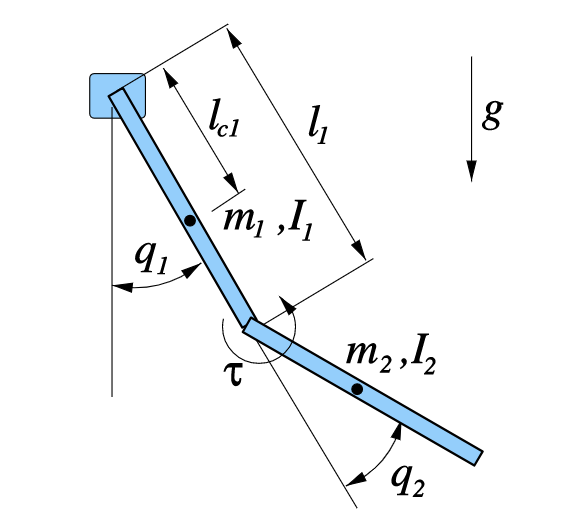
\includegraphics[width=0.45\linewidth]{parameters.png}
\caption{Acrobot (Modified on the basis of picture from \cite{tedrake})}
\label{fig:acrobot}
\end{figure} \\
\null \quad An acrobot closely resembles the movement of a man, and is an important part of a robot. One of the most popular control task studied for the acrobot is the \textit{swing-up} \cite{spong} task, in which the system must use the elbow torque to move the system into a vertical configuration and then balance. Previous studies have proposed many controllers for the Acrobot, such as energy based controllers \cite{1}\cite{2}, controllers based on partiallinearization \cite{1}\cite{3}, tracking controller \cite{4}, back stepping controller \cite{5}, a controller based on the motion of the real gymnast \cite{6} etc. Though optimal control is a powerful framework for specifying complex behaviors with simple objective functions, the computational tools cannot scale well to systems with state dimension more than four or five \cite{tedrake}. In this project, we attempt to find an optimal control solution that is valid from only a single initial condition, instead of solving for the optimal feedback controller for the entire state space. Thus, we represent the optimal control solution as a \textit{trajectory}, \textbf{x($\cdot$)}, \textbf{u($\cdot$)} rather than a feedback control function. \\
\null\quad The rest of this report is organized as follows: In Section~\ref{Dynamics of the Acrobot}, we derive the motion equation of the acrobot using standard, manipulator equation form. In Section~\ref{Optimization}, we set up the Lagrangian equations and derive necessary conditions for the trajectory optimization problem. In Section~\ref{results}, we present the results and runtime analysis of the trajectory optimization solutions. In Section~\ref{rf}, we apply a cutting-edge neural network model - the reinforcement learning algorithm to solve the trajectory optimization problem and compare the performance with traditional methods.

\section{Dynamics of the Acrobot} \label{Dynamics of the Acrobot}
\quad In Figure~\ref{fig:acrobot}, $q_1$ is the shoulder joint angle, $q_2$ is the relative joint angle at the elbow. With the notations in Figure~\ref{fig:acrobot} and let $\mathbf u=[u_1, u_2]^T$ represent the torque applied to the shoulder and the elbow respectively, $\mathbf q = [q_1, q_2]^T$, $\mathbf {\dot q} = [\dot{q_1}, \dot{q_2}]^T$and $\mathbf {\ddot q} = [\ddot{q_1}, \ddot{q_2}]^T$, we can derive the equations of motion in standard, manipulator equation form (for fully actuated acrobot):

\begin{align} \label{eq:manipulator}
\mathbf{H}(\mathbf q) \mathbf{\ddot{q}} +  \mathbf {C( q,\dot{ q})}\mathbf{\dot{q}} + {\mathbf G}(\mathbf q) = \mathbf {Bu} 
\end{align}
where
\begin{align}
{\mathbf H}(\mathbf q) &= \begin{bmatrix} I_1 + I_2 + m_2 l_1^2 + 2m_2 l_1 l_{c2}
  c_2 & I_2 + m_2 l_1 l_{c2} c_2 \\ I_2 + m_2 l_1 l_{c2} c_2 & I_2
  \end{bmatrix},\label{eq:Hacrobot} \nonumber \\
  \mathbf {C(q,\dot{q})} &= \begin{bmatrix} -2 m_2
  l_1 l_{c2} s_2 \dot{q}_2 & -m_2 l_1 l_{c2} s_2 \dot{q}_2 \\ m_2 l_1
  l_{c2} s_2 \dot{q}_1 & 0 \end{bmatrix}, \nonumber \\
{\mathbf G}(\mathbf q) &= \begin{bmatrix} m_1 g l_{c1}s_1 + m_2 g (l_1 s_1 + l_{c2}s_{1+2})
\\ m_2 g l_{c2} s_{1+2} \end{bmatrix}, \nonumber\\
  {\mathbf B} &= \begin{bmatrix} 1 & 0 \\ 0 & 1 \end{bmatrix}. \nonumber
\end{align}
 Note that to model an underactuated acrobot with an actuator at the elbow, we can adjust the above system by simply changing $\mathbf B$ to $\begin{bmatrix} 0 & 0 \\ 0 & 1 \end{bmatrix}$.\\
\null \quad In the next steps we derive the deterministic dynamics from the above motion equations. First, we add frictions $f$ to the system:

\begin{equation} \label{eq:addfriction}
\mathbf {Bu} = \mathbf {B\hat{u}}-f \mathbf{\dot{q}}
\end{equation}
Substituting equation~(\ref{eq:addfriction}) into the right hand side of equation~(\ref{eq:manipulator}), we get:
\begin{equation}
\mathbf{H}(\mathbf q) \mathbf{\ddot{q}} +  \mathbf {C(q,\dot{q})} \mathbf{\dot{q}} + {\mathbf G}(\mathbf q) =  \mathbf {B\hat{u}}-f \mathbf{\dot{q}}
\end{equation}
Afterwards, $\mathbf{\ddot{q}}$ can be calculated as:
\begin{align}
\mathbf{\ddot{q}} &= \mathbf{H(q)}^{-1}[\mathbf{-C(q,\dot{q})\dot{q}-G(q)}+\mathbf {B\hat{u}}-f\mathbf{\dot{q}}] \nonumber \\
&= \mathbf{H(q)}^{-1}[-\mathbf{C(q,\dot{q})\dot{q}}-\mathbf{G(q)}-f\mathbf{\dot{q}}]+\mathbf{H(q)^{-1}B\hat{u}}
\end{align}
Let \textbf{x} = $[q_1, q_2, \dot{q_1}, \dot{q_2}]^T$, we can calculate its derivative with respect to time:
\begin{equation} \label{eq:x_dot}
\mathbf {\dot{x}} = \begin{bmatrix} \dot{q_1} \\ \dot{q_2} \\ \ddot{q_1} \\ \ddot{q_2} \end{bmatrix} = \begin{bmatrix} \dot{q_1} \\ \dot{q_2} \\ \mathbf{H(q)}^{-1}[-\mathbf{C(q,\dot{q})\dot{q}}-\mathbf{G(q)}-f\mathbf{\dot{q}}] \end{bmatrix} 
+ \begin{bmatrix} \mathbf 0 \\ \mathbf 0 \\ \mathbf{H(q)^{-1}B} \end{bmatrix} \mathbf{\hat{u}},
\end{equation}  in the format of 
$
\mathbf{\dot{x}} = \mathbf{f}(\mathbf{ x, u}) = \mathbf{a} + \mathbf {b u}
$. \\
\null \quad For the simplicity of computation, we set all constant values (i.e., $I_1, I_2$, $l_1, l_2, m_1, m_2$, $l_{c1}, l_{c2}$, $c_1$, $c_2$) equal to $1$, hence the matrix $\mathbf{H(q)}$, $\mathbf{C(q,\dot{q})}$ and $\mathbf{G(q)}$ in equation~\ref{eq:x_dot} can be rewritten as:
\begin{align}
\mathbf{H(q)} &= \begin{bmatrix} 3+2\cos(q_2) & 1+\cos(q_2) \\ 1+\cos(q_2) & 1 \end{bmatrix} \nonumber \\
\mathbf{C(q,\dot{q})} &=\begin{bmatrix} -2\sin(q_2)\dot{q_2} & -\sin(q_2)\dot{q_2} \\ \sin(q_2)\dot{q_1} & 0 \end{bmatrix} \nonumber \\
\mathbf{G(q)} &=\begin{bmatrix} g\sin(q_1)+g(\sin(q_1)+\sin(q_1+q_2)) \\ g\sin(q_1+q_2) \end{bmatrix} \nonumber
\end{align}
And hence
\begin{align}
\mathbf{-C(q,\dot{q})\dot{q}-G(q) } &= \begin{bmatrix} 2\sin(q_2)\dot{q_1}\dot{q_2}+\sin(q_2)\dot{q_2}^2 \\ -\sin(q_2)\dot{q_1}^2 \end{bmatrix}-\begin{bmatrix} g\sin(q_1)+g(\sin(q_1)+\sin(q_1+q_2)) \\ g\sin(q_1+q_2) \end{bmatrix} \nonumber \\
&=  \begin{bmatrix} \dot{q_2}(2\dot{q_1}+\dot{q_2})\sin(q_2)-2g \sin(q_1)-g\sin(q_1+q_2) \\ -\dot{q_1}^2\sin(q_2)-g\sin(q_1+q_2) \end{bmatrix} \nonumber
\end{align}

By the end of this section we have derived the $\mathbf{\dot{x}}$ (Equation~\ref{eq:x_dot}). By applying $\mathbf{\dot{x}}$ to the deterministic dynamic function $\mathbf x[n+1] = \mathbf x[n] + \mathbf {\dot{x}}[n]$, we can calculate the next state given previous state and the torque, and hence we have derived the dynamics of the acrobot.

\section{Trajectory Optimization} \label{Optimization}
\subsection{Cost Function}
\quad Define the cost function as
\begin{align}\label{eq:cost}
g(\mathbf q, \mathbf u) = \frac{r}{2}(u_1 + u_2)^2 + 1 - \exp(-k\cos(q_1) + k\cos(q_2) - 2k),
\end{align} where $r, k$ are constants. The reason we choose to use cosine function ($\pm \cos(\cdot)$) as the cost function at both links $q_1$ and $q_2$ is to take advantage of the monotonic and cyclical characteristics of the cosine function. As we can see from Figure~\ref{fig:cost}, $x = \pi$ (the red point) is a global minima, and no matter where we start within the boundary $[0, 2\pi]$ (the purple points), it will converge to $x = \pi$ and will end up with the global minima. \\
\begin{figure}[H]
\centering
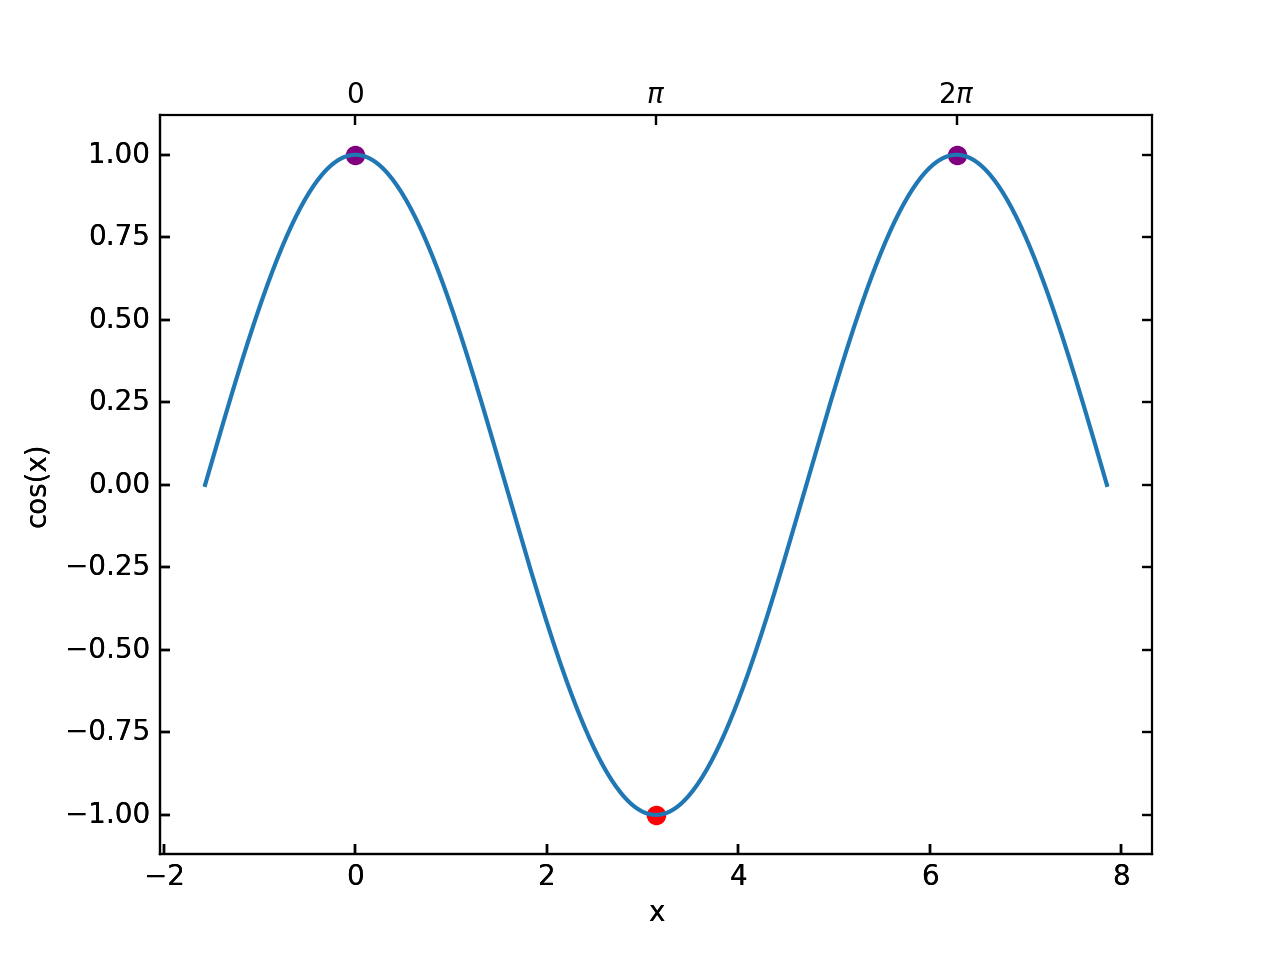
\includegraphics[width=0.8\linewidth]{exp_cosx.png}
\caption{$\cos(x)$}
\label{fig:cost}
\end{figure}

Figure~\ref{fig:cost_contour} demonstrates the distribution of the 2-dimensional cost function in contour. The two purple spots are global minima, and starting from the point ($0, 0$), we can arrive at one of the global minima no matter which direction we choose to go.

\begin{figure}[H]
\begin{center}
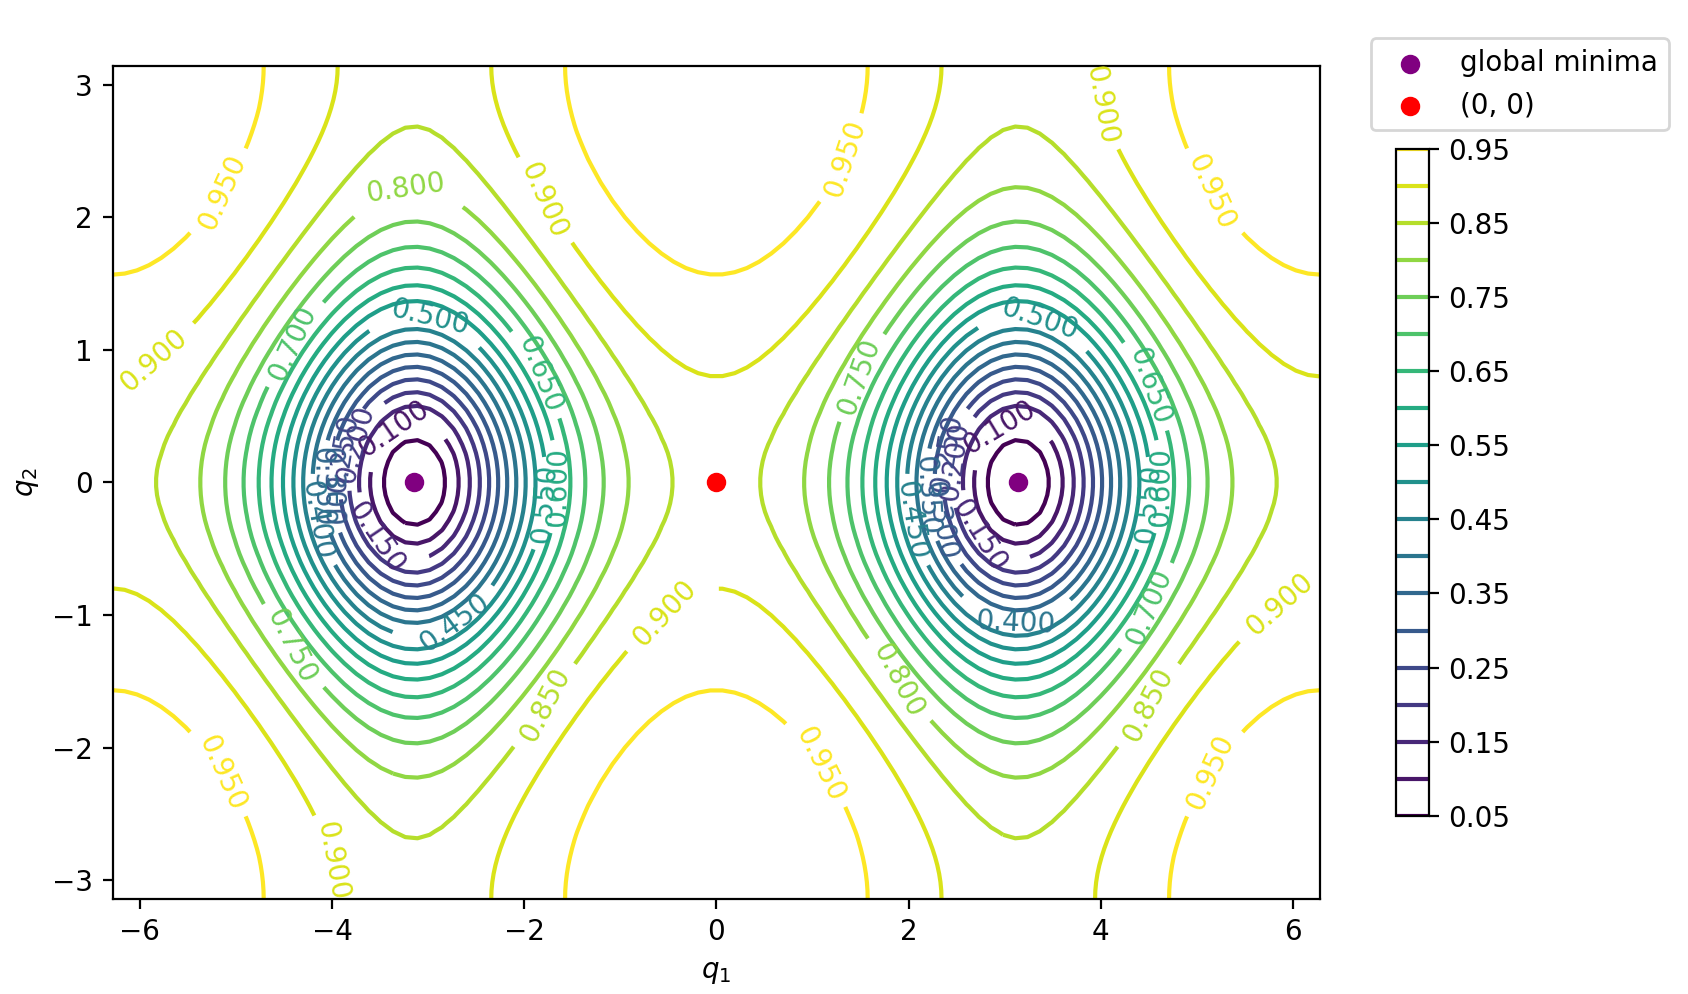
\includegraphics[width=1.1\linewidth]{cost_contour.png}
\caption[caption]{Contour of $1-\exp(-\cos(q_1) + \cos(q_2)-2)$}
\label{fig:cost_contour}
\end{center}
\end{figure}
 In our settings (see Figure~\ref{fig:acrobot}), $q_1$ is the angle between the upper arm and the vertical line going downwards and $q_2$ is the angle between the upper arm and the lower arm. At the beginning of the swing-up process, both arms were hanging downwards so $q_1 = 0$ and $q_2 = 0$ is the starting state. Afterwards, the torque goes into effect so that $q_1$ either increases towards $\pi$ or decreases towards $-\pi$, and the global minima can be achieved in both cases. In other words, the arms can swing up either clockwisely or counter-clockwisely, and both will end up in the desired state. 
\subsection{Lagrangian Constrained Optimization} \label{Lag}
 \quad The constrained trajectory optimization problem in discrete time can be described as below:
\begin{align} & \text{minimize}_{\mathbf x_1,...,\mathbf x_N, u_0,...,u_{N-1}} \sum_{n=0}^{N-1} g(\mathbf x[n], \mathbf u[n]), \nonumber\\
  & \text{subject to} \quad \mathbf x[n+1] = \mathbf {f_d}(\mathbf x[n], \mathbf u[n]) = \mathbf x[n] + \mathbf f(\mathbf x[n], \mathbf u[n]). 
\end{align}
We use Lagrange multipliers to derive the necessary conditions for
our trajectory optimization problem:
\begin{equation}
L(\mathbf x[\cdot],\mathbf u[\cdot],\mathbf \lambda[\cdot]) = \sum_{n=0}^{N-1} g(\mathbf x[n], \mathbf u[n]) +
  \sum_{n=0}^{N-1} \lambda^T[n] \left(\mathbf{f_d}(\mathbf x[n],\mathbf u[n]) - \mathbf x[n+1]\right)
\end{equation}
Take first-order derivatives with respect to $\lambda[\cdot]$, $\mathbf x[\cdot]$ and $\mathbf u[\cdot]$ and set the values equal to $0$'s:

 \begin{align} \forall n\in[0,N-1], \frac{\partial {L}}{\partial{\lambda[n]}} &= \mathbf{f_d}(\mathbf x[n], u[n]) - \mathbf x[n+1] = 0 \nonumber \\ \Rightarrow \mathbf x[n+1] &= \mathbf{f_d}(\mathbf x[n], \mathbf u[n])  \label{eq:dynamic_eq}
 \\
    \forall n\in[0,N-2], \frac{\partial{L}}{\partial \mathbf x[n]} &= \frac{\partial{g(\mathbf x[n],\mathbf u[n])}}{\partial \mathbf x} + \lambda^T[n] \frac{\partial{\mathbf{f_d}(\mathbf x[n],\mathbf u[n])}}{\partial \mathbf x} - \lambda^T[n-1] = 0 \nonumber \\
    \quad \Rightarrow \lambda[n-1] &= \frac{\partial{g(\mathbf x[n],\mathbf u[n])}}{\partial \mathbf x}^T + \frac{\partial{\mathbf{f_d}(\mathbf x[n],\mathbf u[n])}}{\partial \mathbf x}^T \lambda[n]. \label{eq:lambda_i}\\
    \frac{\partial{L}}{\partial \mathbf x[N]} &= -\lambda[N-1] = 0 \nonumber \\ \Rightarrow \lambda[N-1] &= 0 \label{eq:lambda_N}\\
    \forall n\in[0,N-1], \frac{\partial{L}}{\partial \mathbf u[n]} &= \frac{\partial{g(\mathbf x[n]}, \mathbf u[n])}{\partial \mathbf u} + \lambda^T[n] \frac{\partial{\mathbf{f_d}(\mathbf x[n], u[n])}}{\partial \mathbf u} = 0. \label{eq:dldu}
  \end{align}
  
Specifically, 
\begin{align}
\frac{\partial g(\mathbf x[n],\mathbf u[n])}{\partial \mathbf x[n]} &= \begin{bmatrix} -\exp(-k\cos(q_1) + k\cos(q_2) - 2k)\sin(q_1)\\ \exp(-k\cos(q_1) + k\cos(q_2) - 2k)\sin(q_2) \\0\\0 \end{bmatrix}\nonumber \\
\frac{\partial g(\mathbf x[n],\mathbf u[n])}{\partial \mathbf u[n]} &= ru \nonumber \\
\frac{\partial{\mathbf{f_d}(\mathbf x[n],\mathbf u[n])}}{\partial \mathbf x} &= \begin{bmatrix} \mathbf 0 & \mathbf I \\ - \mathbf H^{-1} \frac{{\partial \mathbf G}}{{\partial \mathbf q}}   & -\mathbf H^{-1} {(\mathbf C+ \mathbf I f)}  \end{bmatrix} \nonumber \\
\frac{\partial{\mathbf{f_d}(\mathbf x[n], u[n])}}{\partial \mathbf u} & =  \begin{bmatrix} \mathbf 0 \\ \mathbf 0 \\ \mathbf{H(q)^{-1}B} \end{bmatrix} \nonumber
\end{align}
where 
\begin{align}
\frac{{\partial \mathbf G}}{{\partial \mathbf q}} = \begin{bmatrix} 2g\cos(q_1) + g\cos(q_1+q_2) & g\cos(q_1+q_2)\\
g\cos(q_1+q_2) & g\cos(q_1+q_2) \end{bmatrix} \nonumber
\end{align}
The optimal trajectory should satisfy the conditions that set the above derivatives all equal to zero. \\
\null \quad We tried to solve the above equations using different numerical methods. At first, we used a brute force method that solves all unknowns at one time, but the result failed to converge. With a deeper understanding of the relationship between the variables, we realized what we are looking for is a series of torque $\mathbf{u}[\cdot]$, and the other unknowns can be computed by dynamic functions. Hence, a better way to solve for the unknowns is back-propagation as follows:\\
\null \quad First, suppose we have a series of torques $\mathbf{u}[\cdot]$ that is randomly generated from a normal distribution. Since we already know the initial condition $\mathbf x[0]$, we can infer $\mathbf x[1]$ by Equation~\ref{eq:dynamic_eq}, which is the dynamic equation. In the same manner, we can infer the next state from current state, and thus we can compute $\mathbf x[2], \mathbf x[3], ..., $ $\mathbf x[N-1]$ sequentially. Then we compute the series of $\mathbf \lambda[\cdot]$ in a reverse order: since $\lambda[N-1] = 0$ (Equation~\ref{eq:lambda_N}) and we already know the sequence $\mathbf x[\cdot]$ and $\mathbf u[\cdot]$, by Equation~\ref{eq:lambda_i} we can infer $\lambda[N-1]$. Similarly, we can compute $\lambda[N-2], ..., \lambda[0]$ sequentially.\\
\null \quad Recall that our goal is to find a sequence of torques $\mathbf u[\cdot]$ that satisfies the equation system Equation~\ref{eq:dynamic_eq}, Equation~\ref{eq:lambda_i}, Equation~\ref{eq:lambda_N} and Equation~\ref{eq:dldu}. Now we have reduced the complicated problem with a bunch of unknowns to a typical root-finding one, with the help of the sequential relationship within $\mathbf x[\cdot]$ and $\mathbf \lambda[\cdot]$. Thus we can solve for $\mathbf u[\cdot]$ using Newton's method or other root finding methods.

 \subsection{Chebyshev Approximation}
\quad Theoretically, the torque should change smoothly with time, and hence the values of $\mathbf u[\cdot]$ should be very similar at adjacent time points if the time step is small enough. Therefore, it might be a waste to optimize all of $\mathbf u[\cdot]$ individually, considering the large number of time points we care about. To reduce the dimensions of this problem, we tried to approximate the torque values $\mathbf u[\cdot]$ using polynomial interpolation. The basic idea of polynomial interpolation is to fit a polynomial curve $g(t)$ to the torque values $\mathbf u[\cdot]$ at selected time points.\\
\null \quad In order to minimize the approximation error, we use Chebyshev interpolation \cite{chebyshev}, which is an orthogonal collocation method. In general, Chebyshev interpolation method chooses sample points at Chebyshev points $c_j$ that are calculated using the equation below:
\begin{equation} \label{cheby}
c_j = \cos \left( \frac{(2j - 1)\pi}{2n} \right), j = 1, . . . , n
 \end{equation}
where $n$ is the order of Chebyshev polynomial. By approximating the torque with a polynomial function of time,  now we can describe the torque with as small as $n$ variables instead of a large number of time steps. Moreover, we no longer need to optimize the torque values $\mathbf u[\cdot]$ at each time step, but only need to optimize the torque values $\mathbf w[\cdot]$ at selected Chebyshev points $\mathbf c[\cdot]$. \\
\null \quad To include Chebyshev interpolation in our implementation, we first choose the initial torque values $\mathbf w[\cdot]$ at Chebyshev points $\mathbf c[\cdot]$, and generate the polynomial function $g(t, \mathbf w, \mathbf c)$ with Lagrangian polynomial method \cite{lagrange_interpolation}:
\begin{align} \label{eq:l_i}
 & g(t, \mathbf w, \mathbf c) =\sum_{j=1}^n w_jl_j(t), \nonumber \\
\text{where} \quad
& l_j(t) =\frac{t-c_1}{c_j-c_1}  ... \frac{x-c_{j-1}}{c_j-c_{j-1}} \cdot \frac{x-c_{j+1}}{c_j-c_{j+1}} ...  \frac{x-c_n}{c_j-c_n} \nonumber \\
\end{align}

With $g(t, \mathbf w, \mathbf c)$, we can compute the torque values at each time step $\mathbf u[\cdot]$. Following the steps described in Section~\ref{Lag} we can derive the gradient $\frac{\partial L}{\partial \mathbf u[\cdot]}$. The gradient $\frac{\partial L}{\partial \mathbf w}$ can be calculated with the formula below:
\begin {align}
\frac{\partial L}{\partial \mathbf w} &= \sum_{i = 0}^T g_w(t,\mathbf w, \mathbf c)^T\frac{\partial L}{\partial \mathbf u[i]}, 
\end {align}
where \begin{align}g_w(t,\mathbf w, \mathbf c) & = \begin{bmatrix} l_1(t) \\ l_2(t)\\ ... \\l_n(t) \end{bmatrix}. \nonumber \end{align}
$l_i(t)$ is defined in Equation~\ref{eq:l_i} and $T$ is total number of discrete time steps.
 \subsection{Linear Quadratic Regulator (LQR)}
\null \quad A different way from Lagrangian Constrained Optimization is to use the optimal feedback controller such as Linear Quadratic Regulator (LQR), so long as we can rewrite the cost function in a quadratic form:
\begin{align}
J(\mathbf x_0) =
\int_0^\infty \left[ \mathbf x^T(t) {\mathbf Q} \mathbf x(t) + \mathbf u^T(t) {\mathbf R} \mathbf u(t) \right]dt, \nonumber \\
\text{where}
\quad \mathbf x(0)=\mathbf x_0, {\mathbf Q}={\mathbf Q}^T>0, {\mathbf R}={\mathbf R}^T>0.
\end{align}
Then the optimal control sequence minimizing the cost is given by: 
\begin{align}
\mathbf u(t) &= -\mathbf {Fx}(t), \nonumber\\
\text{where} \quad \mathbf F &= (\mathbf R + \mathbf B^T\mathbf{PB})^{-1}(\mathbf B^T\mathbf{PA} + \mathbf N^T) \nonumber \\
\text{and} \quad \mathbf P &=  \mathbf A^T \mathbf{PA} - \mathbf A^T \mathbf{PB}(\mathbf R+\mathbf B^T \mathbf{PB})^{-1}\mathbf B^T \mathbf{PA} + \mathbf Q 
\end{align}
Detailed explanation please refer to \cite{sontag}.

\section{Results} \label{results}
\subsection{Fully-actuated Acrobot}
\quad To start, we experimented with a fully-actuated acrobot with two actuators, one at the shoulder and the other at the elbow. We tried a variety of ways to solve for the optimal trajectory using Lagrangian constrained optimization method  (as described in Section~\ref{Lag}): Firstly, we tried to solve all the unknowns at once using brute force solver which failed to converge. Then we used the back-propagation way to reduce the number of unknowns and the \texttt{root} function of \texttt{scipy.optimize} module to solve for $\mathbf u$, but sometimes it got to the local maxima instead of minima. Finally we used \texttt{minimum} function of \texttt{scipy.optimize} module and successfully solved for $\mathbf u$ that minimizes our cost function.\\
\null \quad As a warm-up practice for the swing-up task, we solved the stabilization problem first. Using Lagrangian constrained optimization method, we successfully found the trajectory for the fully-actuated acrobot to get back to its balance state ($q_1 = \pi$, $q_2 = 0$) after its upper-arm deviated by an angle of $0.1$ (i.e., $q_1= \pi - 0.1$, $q_2 = 0$) (Figure~\ref{fig:full_stablization}).
\begin{figure}[H]
\begin{center}
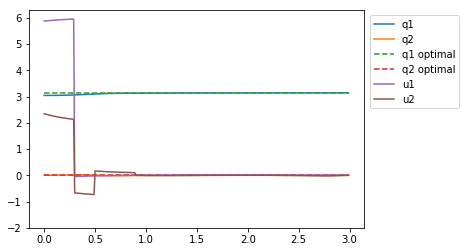
\includegraphics[width=0.8\linewidth]{full_stablization.png}
\caption[caption]{Fully-actuated Stabilization}
\label{fig:full_stablization}
\end{center}
\end{figure}

Then we tried to untangle the swing-up problem of a fully-actuated acrobot. The \texttt{minimum} function of \texttt{scipy.optimize} gets easily trapped in local minima, so we found it difficult to converge to a swing-up trajectory without a good initial value of $\mathbf u$. After many attempts, we finally found a series of initial $\mathbf u$ that can lead to the global minima and can finish the swing-up process (Figure~\ref{fig:full_swingup}).

\begin{figure}[H]
\begin{center}
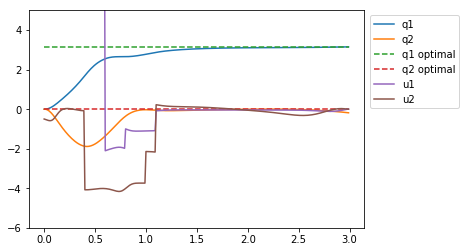
\includegraphics[width=0.8\linewidth]{full_swingup.png}
\caption[caption]{Fully-actuated Swing-up}
\label{fig:full_swingup}
\end{center}
\end{figure}

\subsection{Underactuated Acrobot}
\quad As stated in Section~\ref{Dynamics of the Acrobot}, the dynamic function of underactuated acrobots is identical to that of fully-actuated acrobots except the matrix $\mathbf B = \begin{bmatrix} 0 & 0 \\ 0 & 1 \end{bmatrix}$ instead of $\begin{bmatrix} 1 & 0 \\ 0 & 1\end{bmatrix}$. 
\subsubsection{Stabilization}
\subsubsection{Swing up}
\begin{figure}[H]
\begin{center}
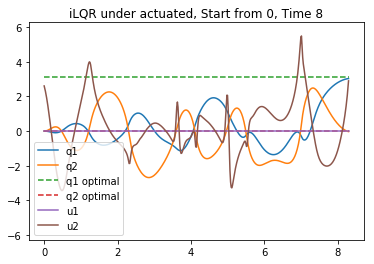
\includegraphics[width=0.6\linewidth]{under_swingup.png}
\caption[caption]{Underactuated Swing-up}
\label{fig:under_swingup}
\end{center}
\end{figure}
\section{Reinforcement Learning} \label{rf}

\newpage
\medskip

\printbibliography
\end{document} to your LaTeX file where you want your
% title page.
%
%%%%%%%%%%%%%%%%%%%%%%%%%%%%%%%%%%%%%%%%%
%\title{Title page with logo}





%----------------------------------------------------------------------------------------
%	PACKAGES AND OTHER DOCUMENT CONFIGURATIONS
%----------------------------------------------------------------------------------------

\documentclass[12pt]{article}
\usepackage[english]{babel}
\usepackage{amsmath}
\usepackage{graphicx}
\usepackage[colorinlistoftodos]{todonotes}
\usepackage{hyperref}
\usepackage[utf8]{inputenc}
\usepackage[backend=bibtex,style=numeric,autocite=plain,sorting=none]{biblatex}
\usepackage{color}
\usepackage{listings}
\usepackage{xcolor}
\usepackage{xparse}
\usepackage{float}

\definecolor{purp}{rgb}{0.6,0.3,0.9}
\addbibresource{citations.bib} %Imports bibliography file

\begin{document}

\begin{titlepage}

\newcommand{\HRule}{\rule{\linewidth}{0.5mm}} % Defines a new command for the horizontal lines, change thickness here

\center % Center everything on the page
 
 %----------------------------------------------------------------------------------------
%	TITLE SECTION
%----------------------------------------------------------------------------------------
\HRule \\[0.4cm]
{\Large \bfseries Optimization in Robotics (Acrobot) Control}\\[0.4cm] % Title of your document
\HRule \\[1.2cm]

%----------------------------------------------------------------------------------------
%	HEADING SECTIONS
%----------------------------------------------------------------------------------------

\textsc{\LARGE Harvard University}\\[1.2cm] % Name of your university/college
\textsc{\Large AM205 Advanced Scientific Computing: Numerical Methods}\\[0.8cm] % Major heading such as course name
\textsc{\large Final Project Report}\\[1.2cm] % Minor heading such as course title


%----------------------------------------------------------------------------------------
%	AUTHOR SECTION
%----------------------------------------------------------------------------------------

\begin{minipage}{0.4\textwidth}
\begin{flushleft} \large
\emph{Authors:}\\
Hengte \textsc{Lin} \\% Your name
Taosha \textsc{Wang}\\
Yifan \textsc{Wang}\\
\end{flushleft}
\end{minipage}
~
\begin{minipage}{0.4\textwidth}
\begin{flushright} \large
\emph{Professor:} \\

Chris H. \textsc{Rycroft} % Supervisor's Name
\end{flushright}
\end{minipage}\\[1cm]

% If you don't want a supervisor, uncomment the two lines below and remove the section above
%\Large \emph{Author:}\\
%John \textsc{Smith}\\[3cm] % Your name

%----------------------------------------------------------------------------------------
%	DATE SECTION
%----------------------------------------------------------------------------------------

{\large \today}\\[1cm] % Date, change the \today to a set date if you want to be precise

%----------------------------------------------------------------------------------------
%	LOGO SECTION
%----------------------------------------------------------------------------------------


\includegraphics[width=0.29\linewidth]{logo.png}\\[1cm] % Include a department/university logo - this will require the graphicx package
 
%----------------------------------------------------------------------------------------

\vfill % Fill the rest of the page with whitespace

\end{titlepage}

%Project motivation: what problem are you trying to solve? What has been
%done before in this area? If appropriate, cite relevant books and papers.

%? 24 points ? Project methods and results: what mathematics and code did you develop
%for your problem? Where appropriate, did you consider mathematical analyses of
%your approach? Is the code that you developed correct?

%? 6 points ? Project conclusions: did you solve what you set out to do? What are
%possible limitations and problems with your approach? How you could you develop
%the project further?
%? 18 points ? Project presentation and organization, divided among the following
%categories:
%? write-up clearly written with good spelling and grammar,
%? figures and tables clear and properly labeled,
%? code well-commented and well-organized.



\begin{abstract}
\quad In this report we describe several algorithms for trajectory optimization of a mechanical system - the acrobot, including the Lagrangian constrained optimization, the linear quadratic regulator, and the Reinforcement Learning algorithm. We tried to solve the stabilization and swing-up problems of the acrobot using each of the algorithms and compared the effectiveness of the results.
\end{abstract}

\section{Introduction}
\quad An \textbf{acrobot}\footnote{A link to an animation of Acrobot: \url{http://www.princeton.edu/~rvdb/WebGL/Acrobot.html} } (in Figure ~\ref{fig:acrobot}) is a planar two-link robotic arm in the vertical plane, typically with an actuator at the elbow (the red point) but no actuator at the shoulder. An acrobot is a typical underactuated robots, which have less actuators than degrees of freedom. The control of underactuated systems has been an interesting topic in robotics industry for it ``gives some reductions of numbers of necessary actuators, of the cost and of the weight of systems" \cite{mingcong}. \\
\begin{figure}[h!]
\centering
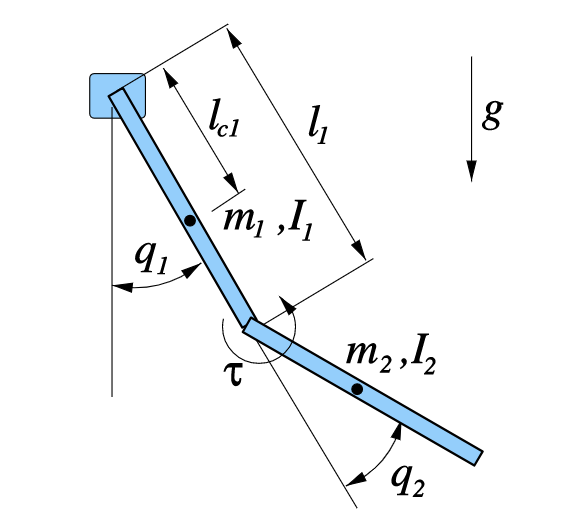
\includegraphics[width=0.45\linewidth]{parameters.png}
\caption{Acrobot (Modified on the basis of picture from \cite{tedrake})}
\label{fig:acrobot}
\end{figure} \\
\null \quad An acrobot closely resembles the movement of a man, and is an important part of a robot. One of the most popular control task studied for the acrobot is the \textit{swing-up} \cite{spong} task, in which the system must use the elbow torque to move the system into a vertical configuration and then balance. Previous studies have proposed many controllers for the Acrobot, such as energy based controllers \cite{1}\cite{2}, controllers based on partiallinearization \cite{1}\cite{3}, tracking controller \cite{4}, back stepping controller \cite{5}, a controller based on the motion of the real gymnast \cite{6} etc. Though optimal control is a powerful framework for specifying complex behaviors with simple objective functions, the computational tools cannot scale well to systems with state dimension more than four or five \cite{tedrake}. In this project, we attempt to find an optimal control solution that is valid from only a single initial condition, instead of solving for the optimal feedback controller for the entire state space. Thus, we represent the optimal control solution as a \textit{trajectory}, \textbf{x($\cdot$)}, \textbf{u($\cdot$)} rather than a feedback control function. \\
\null\quad The rest of this report is organized as follows: In Section~\ref{Dynamics of the Acrobot}, we derive the motion equation of the acrobot using standard, manipulator equation form. In Section~\ref{Optimization}, we set up the Lagrangian equations and derive necessary conditions for the trajectory optimization problem. In Section~\ref{results}, we present the results and runtime analysis of the trajectory optimization solutions. In Section~\ref{rf}, we apply a cutting-edge neural network model - the reinforcement learning algorithm to solve the trajectory optimization problem and compare the performance with traditional methods.

\section{Dynamics of the Acrobot} \label{Dynamics of the Acrobot}
\quad In Figure~\ref{fig:acrobot}, $q_1$ is the shoulder joint angle, $q_2$ is the relative joint angle at the elbow. With the notations in Figure~\ref{fig:acrobot} and let $\mathbf u=[u_1, u_2]^T$ represent the torque applied to the shoulder and the elbow respectively, $\mathbf q = [q_1, q_2]^T$, $\mathbf {\dot q} = [\dot{q_1}, \dot{q_2}]^T$and $\mathbf {\ddot q} = [\ddot{q_1}, \ddot{q_2}]^T$, we can derive the equations of motion in standard, manipulator equation form (for fully actuated acrobot):

\begin{align} \label{eq:manipulator}
\mathbf{H}(\mathbf q) \mathbf{\ddot{q}} +  \mathbf {C( q,\dot{ q})}\mathbf{\dot{q}} + {\mathbf G}(\mathbf q) = \mathbf {Bu} 
\end{align}
where
\begin{align}
{\mathbf H}(\mathbf q) &= \begin{bmatrix} I_1 + I_2 + m_2 l_1^2 + 2m_2 l_1 l_{c2}
  c_2 & I_2 + m_2 l_1 l_{c2} c_2 \\ I_2 + m_2 l_1 l_{c2} c_2 & I_2
  \end{bmatrix},\label{eq:Hacrobot} \nonumber \\
  \mathbf {C(q,\dot{q})} &= \begin{bmatrix} -2 m_2
  l_1 l_{c2} s_2 \dot{q}_2 & -m_2 l_1 l_{c2} s_2 \dot{q}_2 \\ m_2 l_1
  l_{c2} s_2 \dot{q}_1 & 0 \end{bmatrix}, \nonumber \\
{\mathbf G}(\mathbf q) &= \begin{bmatrix} m_1 g l_{c1}s_1 + m_2 g (l_1 s_1 + l_{c2}s_{1+2})
\\ m_2 g l_{c2} s_{1+2} \end{bmatrix}, \nonumber\\
  {\mathbf B} &= \begin{bmatrix} 1 & 0 \\ 0 & 1 \end{bmatrix}. \nonumber
\end{align}
 Note that to model an underactuated acrobot with an actuator at the elbow, we can adjust the above system by simply changing $\mathbf B$ to $\begin{bmatrix} 0 & 0 \\ 0 & 1 \end{bmatrix}$.\\
\null \quad In the next steps we derive the deterministic dynamics from the above motion equations. First, we add frictions $f$ to the system:

\begin{equation} \label{eq:addfriction}
\mathbf {Bu} = \mathbf {B\hat{u}}-f \mathbf{\dot{q}}
\end{equation}
Substituting equation~(\ref{eq:addfriction}) into the right hand side of equation~(\ref{eq:manipulator}), we get:
\begin{equation}
\mathbf{H}(\mathbf q) \mathbf{\ddot{q}} +  \mathbf {C(q,\dot{q})} \mathbf{\dot{q}} + {\mathbf G}(\mathbf q) =  \mathbf {B\hat{u}}-f \mathbf{\dot{q}}
\end{equation}
Afterwards, $\mathbf{\ddot{q}}$ can be calculated as:
\begin{align}
\mathbf{\ddot{q}} &= \mathbf{H(q)}^{-1}[\mathbf{-C(q,\dot{q})\dot{q}-G(q)}+\mathbf {B\hat{u}}-f\mathbf{\dot{q}}] \nonumber \\
&= \mathbf{H(q)}^{-1}[-\mathbf{C(q,\dot{q})\dot{q}}-\mathbf{G(q)}-f\mathbf{\dot{q}}]+\mathbf{H(q)^{-1}B\hat{u}}
\end{align}
Let \textbf{x} = $[q_1, q_2, \dot{q_1}, \dot{q_2}]^T$, we can calculate its derivative with respect to time:
\begin{equation} \label{eq:x_dot}
\mathbf {\dot{x}} = \begin{bmatrix} \dot{q_1} \\ \dot{q_2} \\ \ddot{q_1} \\ \ddot{q_2} \end{bmatrix} = \begin{bmatrix} \dot{q_1} \\ \dot{q_2} \\ \mathbf{H(q)}^{-1}[-\mathbf{C(q,\dot{q})\dot{q}}-\mathbf{G(q)}-f\mathbf{\dot{q}}] \end{bmatrix} 
+ \begin{bmatrix} \mathbf 0 \\ \mathbf 0 \\ \mathbf{H(q)^{-1}B} \end{bmatrix} \mathbf{\hat{u}},
\end{equation}  in the format of 
$
\mathbf{\dot{x}} = \mathbf{f}(\mathbf{ x, u}) = \mathbf{a} + \mathbf {b u}
$. \\
\null \quad For the simplicity of computation, we set all constant values (i.e., $I_1, I_2$, $l_1, l_2, m_1, m_2$, $l_{c1}, l_{c2}$, $c_1$, $c_2$) equal to $1$, hence the matrix $\mathbf{H(q)}$, $\mathbf{C(q,\dot{q})}$ and $\mathbf{G(q)}$ in equation~\ref{eq:x_dot} can be rewritten as:
\begin{align}
\mathbf{H(q)} &= \begin{bmatrix} 3+2\cos(q_2) & 1+\cos(q_2) \\ 1+\cos(q_2) & 1 \end{bmatrix} \nonumber \\
\mathbf{C(q,\dot{q})} &=\begin{bmatrix} -2\sin(q_2)\dot{q_2} & -\sin(q_2)\dot{q_2} \\ \sin(q_2)\dot{q_1} & 0 \end{bmatrix} \nonumber \\
\mathbf{G(q)} &=\begin{bmatrix} g\sin(q_1)+g(\sin(q_1)+\sin(q_1+q_2)) \\ g\sin(q_1+q_2) \end{bmatrix} \nonumber
\end{align}
And hence
\begin{align}
\mathbf{-C(q,\dot{q})\dot{q}-G(q) } &= \begin{bmatrix} 2\sin(q_2)\dot{q_1}\dot{q_2}+\sin(q_2)\dot{q_2}^2 \\ -\sin(q_2)\dot{q_1}^2 \end{bmatrix}-\begin{bmatrix} g\sin(q_1)+g(\sin(q_1)+\sin(q_1+q_2)) \\ g\sin(q_1+q_2) \end{bmatrix} \nonumber \\
&=  \begin{bmatrix} \dot{q_2}(2\dot{q_1}+\dot{q_2})\sin(q_2)-2g \sin(q_1)-g\sin(q_1+q_2) \\ -\dot{q_1}^2\sin(q_2)-g\sin(q_1+q_2) \end{bmatrix} \nonumber
\end{align}

By the end of this section we have derived the $\mathbf{\dot{x}}$ (Equation~\ref{eq:x_dot}). By applying $\mathbf{\dot{x}}$ to the deterministic dynamic function $\mathbf x[n+1] = \mathbf x[n] + \mathbf {\dot{x}}[n]$, we can calculate the next state given previous state and the torque, and hence we have derived the dynamics of the acrobot.

\section{Trajectory Optimization} \label{Optimization}
\subsection{Cost Function}
\quad Define the cost function as
\begin{align}\label{eq:cost}
g(\mathbf q, \mathbf u) = \frac{r}{2}(u_1 + u_2)^2 + 1 - \exp(-k\cos(q_1) + k\cos(q_2) - 2k),
\end{align} where $r, k$ are constants. The reason we choose to use cosine function ($\pm \cos(\cdot)$) as the cost function at both links $q_1$ and $q_2$ is to take advantage of the monotonic and cyclical characteristics of the cosine function. As we can see from Figure~\ref{fig:cost}, $x = \pi$ (the red point) is a global minima, and no matter where we start within the boundary $[0, 2\pi]$ (the purple points), it will converge to $x = \pi$ and will end up with the global minima. \\
\begin{figure}[H]
\centering
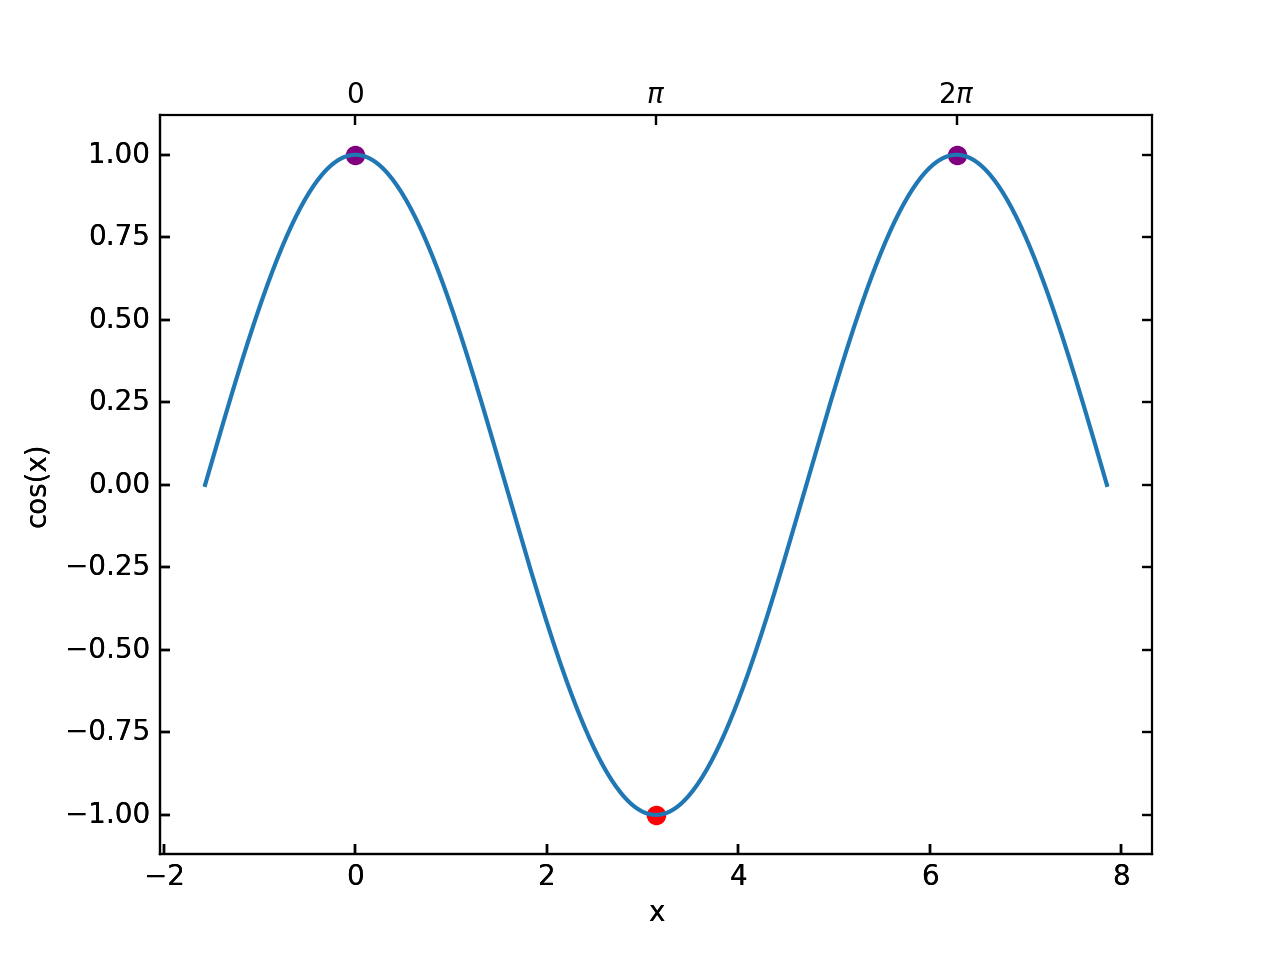
\includegraphics[width=0.8\linewidth]{exp_cosx.png}
\caption{$\cos(x)$}
\label{fig:cost}
\end{figure}

Figure~\ref{fig:cost_contour} demonstrates the distribution of the 2-dimensional cost function in contour. The two purple spots are global minima, and starting from the point ($0, 0$), we can arrive at one of the global minima no matter which direction we choose to go.

\begin{figure}[H]
\begin{center}
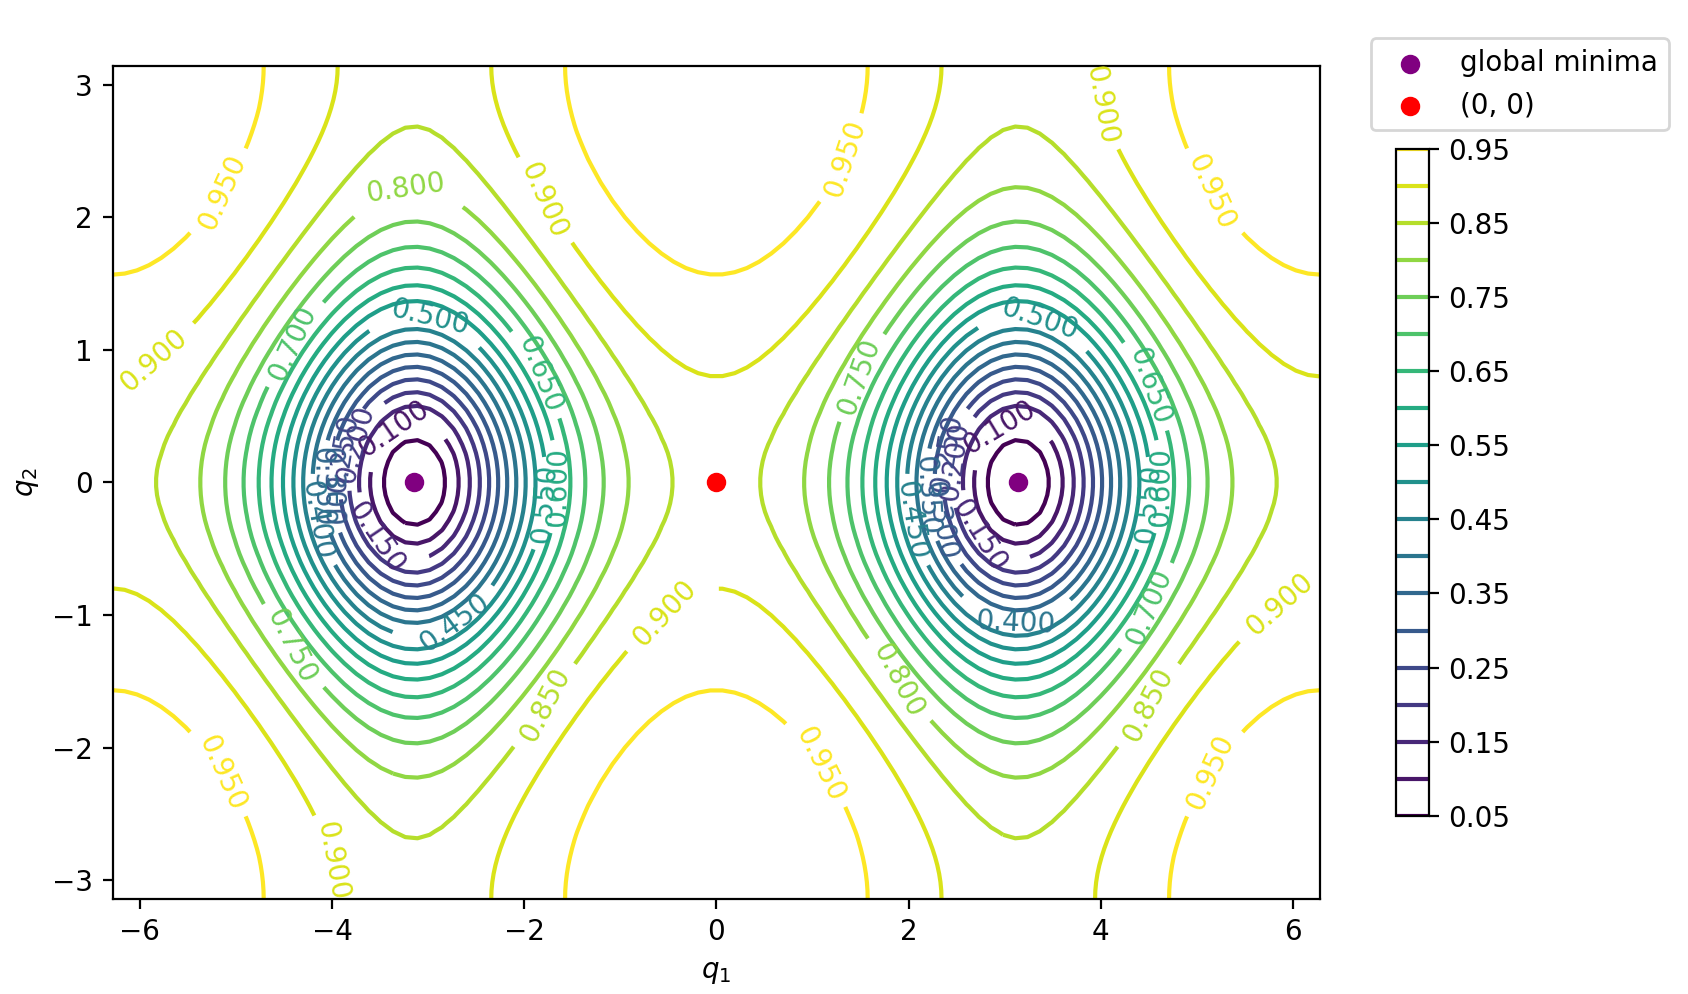
\includegraphics[width=1.1\linewidth]{cost_contour.png}
\caption[caption]{Contour of $1-\exp(-\cos(q_1) + \cos(q_2)-2)$}
\label{fig:cost_contour}
\end{center}
\end{figure}
 In our settings (see Figure~\ref{fig:acrobot}), $q_1$ is the angle between the upper arm and the vertical line going downwards and $q_2$ is the angle between the upper arm and the lower arm. At the beginning of the swing-up process, both arms were hanging downwards so $q_1 = 0$ and $q_2 = 0$ is the starting state. Afterwards, the torque goes into effect so that $q_1$ either increases towards $\pi$ or decreases towards $-\pi$, and the global minima can be achieved in both cases. In other words, the arms can swing up either clockwisely or counter-clockwisely, and both will end up in the desired state. 
\subsection{Lagrangian Constrained Optimization} \label{Lag}
 \quad The constrained trajectory optimization problem in discrete time can be described as below:
\begin{align} & \text{minimize}_{\mathbf x_1,...,\mathbf x_N, u_0,...,u_{N-1}} \sum_{n=0}^{N-1} g(\mathbf x[n], \mathbf u[n]), \nonumber\\
  & \text{subject to} \quad \mathbf x[n+1] = \mathbf {f_d}(\mathbf x[n], \mathbf u[n]) = \mathbf x[n] + \mathbf f(\mathbf x[n], \mathbf u[n]). 
\end{align}
We use Lagrange multipliers to derive the necessary conditions for
our trajectory optimization problem:
\begin{equation}
L(\mathbf x[\cdot],\mathbf u[\cdot],\mathbf \lambda[\cdot]) = \sum_{n=0}^{N-1} g(\mathbf x[n], \mathbf u[n]) +
  \sum_{n=0}^{N-1} \lambda^T[n] \left(\mathbf{f_d}(\mathbf x[n],\mathbf u[n]) - \mathbf x[n+1]\right)
\end{equation}
Take first-order derivatives with respect to $\lambda[\cdot]$, $\mathbf x[\cdot]$ and $\mathbf u[\cdot]$ and set the values equal to $0$'s:

 \begin{align} \forall n\in[0,N-1], \frac{\partial {L}}{\partial{\lambda[n]}} &= \mathbf{f_d}(\mathbf x[n], u[n]) - \mathbf x[n+1] = 0 \nonumber \\ \Rightarrow \mathbf x[n+1] &= \mathbf{f_d}(\mathbf x[n], \mathbf u[n])  \label{eq:dynamic_eq}
 \\
    \forall n\in[0,N-2], \frac{\partial{L}}{\partial \mathbf x[n]} &= \frac{\partial{g(\mathbf x[n],\mathbf u[n])}}{\partial \mathbf x} + \lambda^T[n] \frac{\partial{\mathbf{f_d}(\mathbf x[n],\mathbf u[n])}}{\partial \mathbf x} - \lambda^T[n-1] = 0 \nonumber \\
    \quad \Rightarrow \lambda[n-1] &= \frac{\partial{g(\mathbf x[n],\mathbf u[n])}}{\partial \mathbf x}^T + \frac{\partial{\mathbf{f_d}(\mathbf x[n],\mathbf u[n])}}{\partial \mathbf x}^T \lambda[n]. \label{eq:lambda_i}\\
    \frac{\partial{L}}{\partial \mathbf x[N]} &= -\lambda[N-1] = 0 \nonumber \\ \Rightarrow \lambda[N-1] &= 0 \label{eq:lambda_N}\\
    \forall n\in[0,N-1], \frac{\partial{L}}{\partial \mathbf u[n]} &= \frac{\partial{g(\mathbf x[n]}, \mathbf u[n])}{\partial \mathbf u} + \lambda^T[n] \frac{\partial{\mathbf{f_d}(\mathbf x[n], u[n])}}{\partial \mathbf u} = 0. \label{eq:dldu}
  \end{align}
  
Specifically, 
\begin{align}
\frac{\partial g(\mathbf x[n],\mathbf u[n])}{\partial \mathbf x[n]} &= \begin{bmatrix} -\exp(-k\cos(q_1) + k\cos(q_2) - 2k)\sin(q_1)\\ \exp(-k\cos(q_1) + k\cos(q_2) - 2k)\sin(q_2) \\0\\0 \end{bmatrix}\nonumber \\
\frac{\partial g(\mathbf x[n],\mathbf u[n])}{\partial \mathbf u[n]} &= ru \nonumber \\
\frac{\partial{\mathbf{f_d}(\mathbf x[n],\mathbf u[n])}}{\partial \mathbf x} &= \begin{bmatrix} \mathbf 0 & \mathbf I \\ - \mathbf H^{-1} \frac{{\partial \mathbf G}}{{\partial \mathbf q}}   & -\mathbf H^{-1} {(\mathbf C+ \mathbf I f)}  \end{bmatrix} \nonumber \\
\frac{\partial{\mathbf{f_d}(\mathbf x[n], u[n])}}{\partial \mathbf u} & =  \begin{bmatrix} \mathbf 0 \\ \mathbf 0 \\ \mathbf{H(q)^{-1}B} \end{bmatrix} \nonumber
\end{align}
where 
\begin{align}
\frac{{\partial \mathbf G}}{{\partial \mathbf q}} = \begin{bmatrix} 2g\cos(q_1) + g\cos(q_1+q_2) & g\cos(q_1+q_2)\\
g\cos(q_1+q_2) & g\cos(q_1+q_2) \end{bmatrix} \nonumber
\end{align}
The optimal trajectory should satisfy the conditions that set the above derivatives all equal to zero. \\
\null \quad We tried to solve the above equations using different numerical methods. At first, we used a brute force method that solves all unknowns at one time, but the result failed to converge. With a deeper understanding of the relationship between the variables, we realized what we are looking for is a series of torque $\mathbf{u}[\cdot]$, and the other unknowns can be computed by dynamic functions. Hence, a better way to solve for the unknowns is back-propagation as follows:\\
\null \quad First, suppose we have a series of torques $\mathbf{u}[\cdot]$ that is randomly generated from a normal distribution. Since we already know the initial condition $\mathbf x[0]$, we can infer $\mathbf x[1]$ by Equation~\ref{eq:dynamic_eq}, which is the dynamic equation. In the same manner, we can infer the next state from current state, and thus we can compute $\mathbf x[2], \mathbf x[3], ..., $ $\mathbf x[N-1]$ sequentially. Then we compute the series of $\mathbf \lambda[\cdot]$ in a reverse order: since $\lambda[N-1] = 0$ (Equation~\ref{eq:lambda_N}) and we already know the sequence $\mathbf x[\cdot]$ and $\mathbf u[\cdot]$, by Equation~\ref{eq:lambda_i} we can infer $\lambda[N-1]$. Similarly, we can compute $\lambda[N-2], ..., \lambda[0]$ sequentially.\\
\null \quad Recall that our goal is to find a sequence of torques $\mathbf u[\cdot]$ that satisfies the equation system Equation~\ref{eq:dynamic_eq}, Equation~\ref{eq:lambda_i}, Equation~\ref{eq:lambda_N} and Equation~\ref{eq:dldu}. Now we have reduced the complicated problem with a bunch of unknowns to a typical root-finding one, with the help of the sequential relationship within $\mathbf x[\cdot]$ and $\mathbf \lambda[\cdot]$. Thus we can solve for $\mathbf u[\cdot]$ using Newton's method or other root finding methods.

 \subsection{Chebyshev Approximation}
\quad Theoretically, the torque should change smoothly with time, and hence the values of $\mathbf u[\cdot]$ should be very similar at adjacent time points if the time step is small enough. Therefore, it might be a waste to optimize all of $\mathbf u[\cdot]$ individually, considering the large number of time points we care about. To reduce the dimensions of this problem, we tried to approximate the torque values $\mathbf u[\cdot]$ using polynomial interpolation. The basic idea of polynomial interpolation is to fit a polynomial curve $g(t)$ to the torque values $\mathbf u[\cdot]$ at selected time points.\\
\null \quad In order to minimize the approximation error, we use Chebyshev interpolation \cite{chebyshev}, which is an orthogonal collocation method. In general, Chebyshev interpolation method chooses sample points at Chebyshev points $c_j$ that are calculated using the equation below:
\begin{equation} \label{cheby}
c_j = \cos \left( \frac{(2j - 1)\pi}{2n} \right), j = 1, . . . , n
 \end{equation}
where $n$ is the order of Chebyshev polynomial. By approximating the torque with a polynomial function of time,  now we can describe the torque with as small as $n$ variables instead of a large number of time steps. Moreover, we no longer need to optimize the torque values $\mathbf u[\cdot]$ at each time step, but only need to optimize the torque values $\mathbf w[\cdot]$ at selected Chebyshev points $\mathbf c[\cdot]$. \\
\null \quad To include Chebyshev interpolation in our implementation, we first choose the initial torque values $\mathbf w[\cdot]$ at Chebyshev points $\mathbf c[\cdot]$, and generate the polynomial function $g(t, \mathbf w, \mathbf c)$ with Lagrangian polynomial method \cite{lagrange_interpolation}:
\begin{align} \label{eq:l_i}
 & g(t, \mathbf w, \mathbf c) =\sum_{j=1}^n w_jl_j(t), \nonumber \\
\text{where} \quad
& l_j(t) =\frac{t-c_1}{c_j-c_1}  ... \frac{x-c_{j-1}}{c_j-c_{j-1}} \cdot \frac{x-c_{j+1}}{c_j-c_{j+1}} ...  \frac{x-c_n}{c_j-c_n} \nonumber \\
\end{align}

With $g(t, \mathbf w, \mathbf c)$, we can compute the torque values at each time step $\mathbf u[\cdot]$. Following the steps described in Section~\ref{Lag} we can derive the gradient $\frac{\partial L}{\partial \mathbf u[\cdot]}$. The gradient $\frac{\partial L}{\partial \mathbf w}$ can be calculated with the formula below:
\begin {align}
\frac{\partial L}{\partial \mathbf w} &= \sum_{i = 0}^T g_w(t,\mathbf w, \mathbf c)^T\frac{\partial L}{\partial \mathbf u[i]}, 
\end {align}
where \begin{align}g_w(t,\mathbf w, \mathbf c) & = \begin{bmatrix} l_1(t) \\ l_2(t)\\ ... \\l_n(t) \end{bmatrix}. \nonumber \end{align}
$l_i(t)$ is defined in Equation~\ref{eq:l_i} and $T$ is total number of discrete time steps.
 \subsection{Linear Quadratic Regulator (LQR)}
\null \quad A different way from Lagrangian Constrained Optimization is to use the optimal feedback controller such as Linear Quadratic Regulator (LQR), so long as we can rewrite the cost function in a quadratic form:
\begin{align}
J(\mathbf x_0) =
\int_0^\infty \left[ \mathbf x^T(t) {\mathbf Q} \mathbf x(t) + \mathbf u^T(t) {\mathbf R} \mathbf u(t) \right]dt, \nonumber \\
\text{where}
\quad \mathbf x(0)=\mathbf x_0, {\mathbf Q}={\mathbf Q}^T>0, {\mathbf R}={\mathbf R}^T>0.
\end{align}
Then the optimal control sequence minimizing the cost is given by: 
\begin{align}
\mathbf u(t) &= -\mathbf {Fx}(t), \nonumber\\
\text{where} \quad \mathbf F &= (\mathbf R + \mathbf B^T\mathbf{PB})^{-1}(\mathbf B^T\mathbf{PA} + \mathbf N^T) \nonumber \\
\text{and} \quad \mathbf P &=  \mathbf A^T \mathbf{PA} - \mathbf A^T \mathbf{PB}(\mathbf R+\mathbf B^T \mathbf{PB})^{-1}\mathbf B^T \mathbf{PA} + \mathbf Q 
\end{align}
Detailed explanation please refer to \cite{sontag}.

\section{Results} \label{results}
\subsection{Fully-actuated Acrobot}
\quad To start, we experimented with a fully-actuated acrobot with two actuators, one at the shoulder and the other at the elbow. We tried a variety of ways to solve for the optimal trajectory using Lagrangian constrained optimization method  (as described in Section~\ref{Lag}): Firstly, we tried to solve all the unknowns at once using brute force solver which failed to converge. Then we used the back-propagation way to reduce the number of unknowns and the \texttt{root} function of \texttt{scipy.optimize} module to solve for $\mathbf u$, but sometimes it got to the local maxima instead of minima. Finally we used \texttt{minimum} function of \texttt{scipy.optimize} module and successfully solved for $\mathbf u$ that minimizes our cost function.\\
\null \quad As a warm-up practice for the swing-up task, we solved the stabilization problem first. Using Lagrangian constrained optimization method, we successfully found the trajectory for the fully-actuated acrobot to get back to its balance state ($q_1 = \pi$, $q_2 = 0$) after its upper-arm deviated by an angle of $0.1$ (i.e., $q_1= \pi - 0.1$, $q_2 = 0$) (Figure~\ref{fig:full_stablization}).
\begin{figure}[H]
\begin{center}
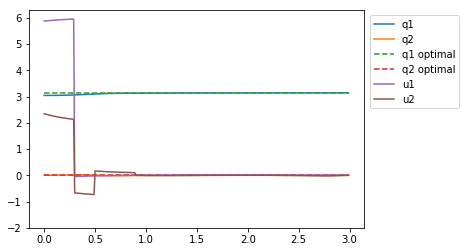
\includegraphics[width=0.8\linewidth]{full_stablization.png}
\caption[caption]{Fully-actuated Stabilization}
\label{fig:full_stablization}
\end{center}
\end{figure}

Then we tried to untangle the swing-up problem of a fully-actuated acrobot. The \texttt{minimum} function of \texttt{scipy.optimize} gets easily trapped in local minima, so we found it difficult to converge to a swing-up trajectory without a good initial value of $\mathbf u$. After many attempts, we finally found a series of initial $\mathbf u$ that can lead to the global minima and can finish the swing-up process (Figure~\ref{fig:full_swingup}).

\begin{figure}[H]
\begin{center}
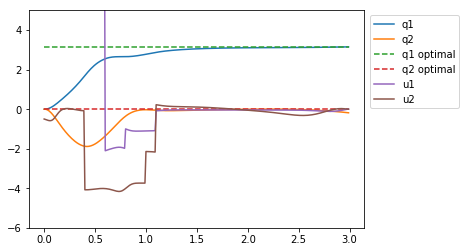
\includegraphics[width=0.8\linewidth]{full_swingup.png}
\caption[caption]{Fully-actuated Swing-up}
\label{fig:full_swingup}
\end{center}
\end{figure}

\subsection{Underactuated Acrobot}
\quad As stated in Section~\ref{Dynamics of the Acrobot}, the dynamic function of underactuated acrobots is identical to that of fully-actuated acrobots except the matrix $\mathbf B = \begin{bmatrix} 0 & 0 \\ 0 & 1 \end{bmatrix}$ instead of $\begin{bmatrix} 1 & 0 \\ 0 & 1\end{bmatrix}$. 
\subsubsection{Stabilization}
\subsubsection{Swing up}
\begin{figure}[H]
\begin{center}
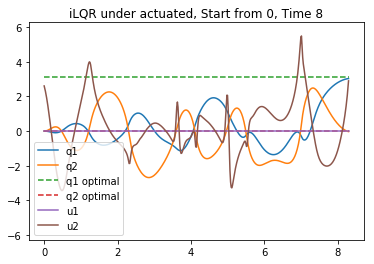
\includegraphics[width=0.6\linewidth]{under_swingup.png}
\caption[caption]{Underactuated Swing-up}
\label{fig:under_swingup}
\end{center}
\end{figure}
\section{Reinforcement Learning} \label{rf}

\newpage
\medskip

\printbibliography
\end{document} to your LaTeX file where you want your
% title page.
%
%%%%%%%%%%%%%%%%%%%%%%%%%%%%%%%%%%%%%%%%%
%\title{Title page with logo}





%----------------------------------------------------------------------------------------
%	PACKAGES AND OTHER DOCUMENT CONFIGURATIONS
%----------------------------------------------------------------------------------------

\documentclass[12pt]{article}
\usepackage[english]{babel}
\usepackage{amsmath}
\usepackage{graphicx}
\usepackage[colorinlistoftodos]{todonotes}
\usepackage{hyperref}
\usepackage[utf8]{inputenc}
\usepackage[backend=bibtex,style=numeric,autocite=plain,sorting=none]{biblatex}
\usepackage{color}
\usepackage{listings}
\usepackage{xcolor}
\usepackage{xparse}
\usepackage{float}

\definecolor{purp}{rgb}{0.6,0.3,0.9}
\addbibresource{citations.bib} %Imports bibliography file

\begin{document}

\begin{titlepage}

\newcommand{\HRule}{\rule{\linewidth}{0.5mm}} % Defines a new command for the horizontal lines, change thickness here

\center % Center everything on the page
 
 %----------------------------------------------------------------------------------------
%	TITLE SECTION
%----------------------------------------------------------------------------------------
\HRule \\[0.4cm]
{\Large \bfseries Optimization in Robotics (Acrobot) Control}\\[0.4cm] % Title of your document
\HRule \\[1.2cm]

%----------------------------------------------------------------------------------------
%	HEADING SECTIONS
%----------------------------------------------------------------------------------------

\textsc{\LARGE Harvard University}\\[1.2cm] % Name of your university/college
\textsc{\Large AM205 Advanced Scientific Computing: Numerical Methods}\\[0.8cm] % Major heading such as course name
\textsc{\large Final Project Report}\\[1.2cm] % Minor heading such as course title


%----------------------------------------------------------------------------------------
%	AUTHOR SECTION
%----------------------------------------------------------------------------------------

\begin{minipage}{0.4\textwidth}
\begin{flushleft} \large
\emph{Authors:}\\
Hengte \textsc{Lin} \\% Your name
Taosha \textsc{Wang}\\
Yifan \textsc{Wang}\\
\end{flushleft}
\end{minipage}
~
\begin{minipage}{0.4\textwidth}
\begin{flushright} \large
\emph{Professor:} \\

Chris H. \textsc{Rycroft} % Supervisor's Name
\end{flushright}
\end{minipage}\\[1cm]

% If you don't want a supervisor, uncomment the two lines below and remove the section above
%\Large \emph{Author:}\\
%John \textsc{Smith}\\[3cm] % Your name

%----------------------------------------------------------------------------------------
%	DATE SECTION
%----------------------------------------------------------------------------------------

{\large \today}\\[1cm] % Date, change the \today to a set date if you want to be precise

%----------------------------------------------------------------------------------------
%	LOGO SECTION
%----------------------------------------------------------------------------------------


\includegraphics[width=0.29\linewidth]{logo.png}\\[1cm] % Include a department/university logo - this will require the graphicx package
 
%----------------------------------------------------------------------------------------

\vfill % Fill the rest of the page with whitespace

\end{titlepage}

%Project motivation: what problem are you trying to solve? What has been
%done before in this area? If appropriate, cite relevant books and papers.

%? 24 points ? Project methods and results: what mathematics and code did you develop
%for your problem? Where appropriate, did you consider mathematical analyses of
%your approach? Is the code that you developed correct?

%? 6 points ? Project conclusions: did you solve what you set out to do? What are
%possible limitations and problems with your approach? How you could you develop
%the project further?
%? 18 points ? Project presentation and organization, divided among the following
%categories:
%? write-up clearly written with good spelling and grammar,
%? figures and tables clear and properly labeled,
%? code well-commented and well-organized.



\begin{abstract}
\quad In this report we describe several algorithms for trajectory optimization of a mechanical system - the acrobot, including the Lagrangian constrained optimization, the linear quadratic regulator, and the Reinforcement Learning algorithm. We tried to solve the stabilization and swing-up problems of the acrobot using each of the algorithms and compared the effectiveness of the results.
\end{abstract}

\section{Introduction}
\quad An \textbf{acrobot}\footnote{A link to an animation of Acrobot: \url{http://www.princeton.edu/~rvdb/WebGL/Acrobot.html} } (in Figure ~\ref{fig:acrobot}) is a planar two-link robotic arm in the vertical plane, typically with an actuator at the elbow (the red point) but no actuator at the shoulder. An acrobot is a typical underactuated robots, which have less actuators than degrees of freedom. The control of underactuated systems has been an interesting topic in robotics industry for it ``gives some reductions of numbers of necessary actuators, of the cost and of the weight of systems" \cite{mingcong}. \\
\begin{figure}[h!]
\centering
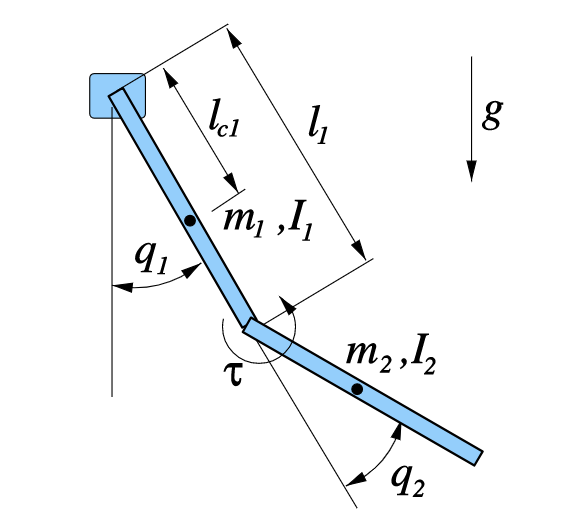
\includegraphics[width=0.45\linewidth]{parameters.png}
\caption{Acrobot (Modified on the basis of picture from \cite{tedrake})}
\label{fig:acrobot}
\end{figure} \\
\null \quad An acrobot closely resembles the movement of a man, and is an important part of a robot. One of the most popular control task studied for the acrobot is the \textit{swing-up} \cite{spong} task, in which the system must use the elbow torque to move the system into a vertical configuration and then balance. Previous studies have proposed many controllers for the Acrobot, such as energy based controllers \cite{1}\cite{2}, controllers based on partiallinearization \cite{1}\cite{3}, tracking controller \cite{4}, back stepping controller \cite{5}, a controller based on the motion of the real gymnast \cite{6} etc. Though optimal control is a powerful framework for specifying complex behaviors with simple objective functions, the computational tools cannot scale well to systems with state dimension more than four or five \cite{tedrake}. In this project, we attempt to find an optimal control solution that is valid from only a single initial condition, instead of solving for the optimal feedback controller for the entire state space. Thus, we represent the optimal control solution as a \textit{trajectory}, \textbf{x($\cdot$)}, \textbf{u($\cdot$)} rather than a feedback control function. \\
\null\quad The rest of this report is organized as follows: In Section~\ref{Dynamics of the Acrobot}, we derive the motion equation of the acrobot using standard, manipulator equation form. In Section~\ref{Optimization}, we set up the Lagrangian equations and derive necessary conditions for the trajectory optimization problem. In Section~\ref{results}, we present the results and runtime analysis of the trajectory optimization solutions. In Section~\ref{rf}, we apply a cutting-edge neural network model - the reinforcement learning algorithm to solve the trajectory optimization problem and compare the performance with traditional methods.

\section{Dynamics of the Acrobot} \label{Dynamics of the Acrobot}
\quad In Figure~\ref{fig:acrobot}, $q_1$ is the shoulder joint angle, $q_2$ is the relative joint angle at the elbow. With the notations in Figure~\ref{fig:acrobot} and let $\mathbf u=[u_1, u_2]^T$ represent the torque applied to the shoulder and the elbow respectively, $\mathbf q = [q_1, q_2]^T$, $\mathbf {\dot q} = [\dot{q_1}, \dot{q_2}]^T$and $\mathbf {\ddot q} = [\ddot{q_1}, \ddot{q_2}]^T$, we can derive the equations of motion in standard, manipulator equation form (for fully actuated acrobot):

\begin{align} \label{eq:manipulator}
\mathbf{H}(\mathbf q) \mathbf{\ddot{q}} +  \mathbf {C( q,\dot{ q})}\mathbf{\dot{q}} + {\mathbf G}(\mathbf q) = \mathbf {Bu} 
\end{align}
where
\begin{align}
{\mathbf H}(\mathbf q) &= \begin{bmatrix} I_1 + I_2 + m_2 l_1^2 + 2m_2 l_1 l_{c2}
  c_2 & I_2 + m_2 l_1 l_{c2} c_2 \\ I_2 + m_2 l_1 l_{c2} c_2 & I_2
  \end{bmatrix},\label{eq:Hacrobot} \nonumber \\
  \mathbf {C(q,\dot{q})} &= \begin{bmatrix} -2 m_2
  l_1 l_{c2} s_2 \dot{q}_2 & -m_2 l_1 l_{c2} s_2 \dot{q}_2 \\ m_2 l_1
  l_{c2} s_2 \dot{q}_1 & 0 \end{bmatrix}, \nonumber \\
{\mathbf G}(\mathbf q) &= \begin{bmatrix} m_1 g l_{c1}s_1 + m_2 g (l_1 s_1 + l_{c2}s_{1+2})
\\ m_2 g l_{c2} s_{1+2} \end{bmatrix}, \nonumber\\
  {\mathbf B} &= \begin{bmatrix} 1 & 0 \\ 0 & 1 \end{bmatrix}. \nonumber
\end{align}
 Note that to model an underactuated acrobot with an actuator at the elbow, we can adjust the above system by simply changing $\mathbf B$ to $\begin{bmatrix} 0 & 0 \\ 0 & 1 \end{bmatrix}$.\\
\null \quad In the next steps we derive the deterministic dynamics from the above motion equations. First, we add frictions $f$ to the system:

\begin{equation} \label{eq:addfriction}
\mathbf {Bu} = \mathbf {B\hat{u}}-f \mathbf{\dot{q}}
\end{equation}
Substituting equation~(\ref{eq:addfriction}) into the right hand side of equation~(\ref{eq:manipulator}), we get:
\begin{equation}
\mathbf{H}(\mathbf q) \mathbf{\ddot{q}} +  \mathbf {C(q,\dot{q})} \mathbf{\dot{q}} + {\mathbf G}(\mathbf q) =  \mathbf {B\hat{u}}-f \mathbf{\dot{q}}
\end{equation}
Afterwards, $\mathbf{\ddot{q}}$ can be calculated as:
\begin{align}
\mathbf{\ddot{q}} &= \mathbf{H(q)}^{-1}[\mathbf{-C(q,\dot{q})\dot{q}-G(q)}+\mathbf {B\hat{u}}-f\mathbf{\dot{q}}] \nonumber \\
&= \mathbf{H(q)}^{-1}[-\mathbf{C(q,\dot{q})\dot{q}}-\mathbf{G(q)}-f\mathbf{\dot{q}}]+\mathbf{H(q)^{-1}B\hat{u}}
\end{align}
Let \textbf{x} = $[q_1, q_2, \dot{q_1}, \dot{q_2}]^T$, we can calculate its derivative with respect to time:
\begin{equation} \label{eq:x_dot}
\mathbf {\dot{x}} = \begin{bmatrix} \dot{q_1} \\ \dot{q_2} \\ \ddot{q_1} \\ \ddot{q_2} \end{bmatrix} = \begin{bmatrix} \dot{q_1} \\ \dot{q_2} \\ \mathbf{H(q)}^{-1}[-\mathbf{C(q,\dot{q})\dot{q}}-\mathbf{G(q)}-f\mathbf{\dot{q}}] \end{bmatrix} 
+ \begin{bmatrix} \mathbf 0 \\ \mathbf 0 \\ \mathbf{H(q)^{-1}B} \end{bmatrix} \mathbf{\hat{u}},
\end{equation}  in the format of 
$
\mathbf{\dot{x}} = \mathbf{f}(\mathbf{ x, u}) = \mathbf{a} + \mathbf {b u}
$. \\
\null \quad For the simplicity of computation, we set all constant values (i.e., $I_1, I_2$, $l_1, l_2, m_1, m_2$, $l_{c1}, l_{c2}$, $c_1$, $c_2$) equal to $1$, hence the matrix $\mathbf{H(q)}$, $\mathbf{C(q,\dot{q})}$ and $\mathbf{G(q)}$ in equation~\ref{eq:x_dot} can be rewritten as:
\begin{align}
\mathbf{H(q)} &= \begin{bmatrix} 3+2\cos(q_2) & 1+\cos(q_2) \\ 1+\cos(q_2) & 1 \end{bmatrix} \nonumber \\
\mathbf{C(q,\dot{q})} &=\begin{bmatrix} -2\sin(q_2)\dot{q_2} & -\sin(q_2)\dot{q_2} \\ \sin(q_2)\dot{q_1} & 0 \end{bmatrix} \nonumber \\
\mathbf{G(q)} &=\begin{bmatrix} g\sin(q_1)+g(\sin(q_1)+\sin(q_1+q_2)) \\ g\sin(q_1+q_2) \end{bmatrix} \nonumber
\end{align}
And hence
\begin{align}
\mathbf{-C(q,\dot{q})\dot{q}-G(q) } &= \begin{bmatrix} 2\sin(q_2)\dot{q_1}\dot{q_2}+\sin(q_2)\dot{q_2}^2 \\ -\sin(q_2)\dot{q_1}^2 \end{bmatrix}-\begin{bmatrix} g\sin(q_1)+g(\sin(q_1)+\sin(q_1+q_2)) \\ g\sin(q_1+q_2) \end{bmatrix} \nonumber \\
&=  \begin{bmatrix} \dot{q_2}(2\dot{q_1}+\dot{q_2})\sin(q_2)-2g \sin(q_1)-g\sin(q_1+q_2) \\ -\dot{q_1}^2\sin(q_2)-g\sin(q_1+q_2) \end{bmatrix} \nonumber
\end{align}

By the end of this section we have derived the $\mathbf{\dot{x}}$ (Equation~\ref{eq:x_dot}). By applying $\mathbf{\dot{x}}$ to the deterministic dynamic function $\mathbf x[n+1] = \mathbf x[n] + \mathbf {\dot{x}}[n]$, we can calculate the next state given previous state and the torque, and hence we have derived the dynamics of the acrobot.

\section{Trajectory Optimization} \label{Optimization}
\subsection{Cost Function}
\quad Define the cost function as
\begin{align}\label{eq:cost}
g(\mathbf q, \mathbf u) = \frac{r}{2}(u_1 + u_2)^2 + 1 - \exp(-k\cos(q_1) + k\cos(q_2) - 2k),
\end{align} where $r, k$ are constants. The reason we choose to use cosine function ($\pm \cos(\cdot)$) as the cost function at both links $q_1$ and $q_2$ is to take advantage of the monotonic and cyclical characteristics of the cosine function. As we can see from Figure~\ref{fig:cost}, $x = \pi$ (the red point) is a global minima, and no matter where we start within the boundary $[0, 2\pi]$ (the purple points), it will converge to $x = \pi$ and will end up with the global minima. \\
\begin{figure}[H]
\centering
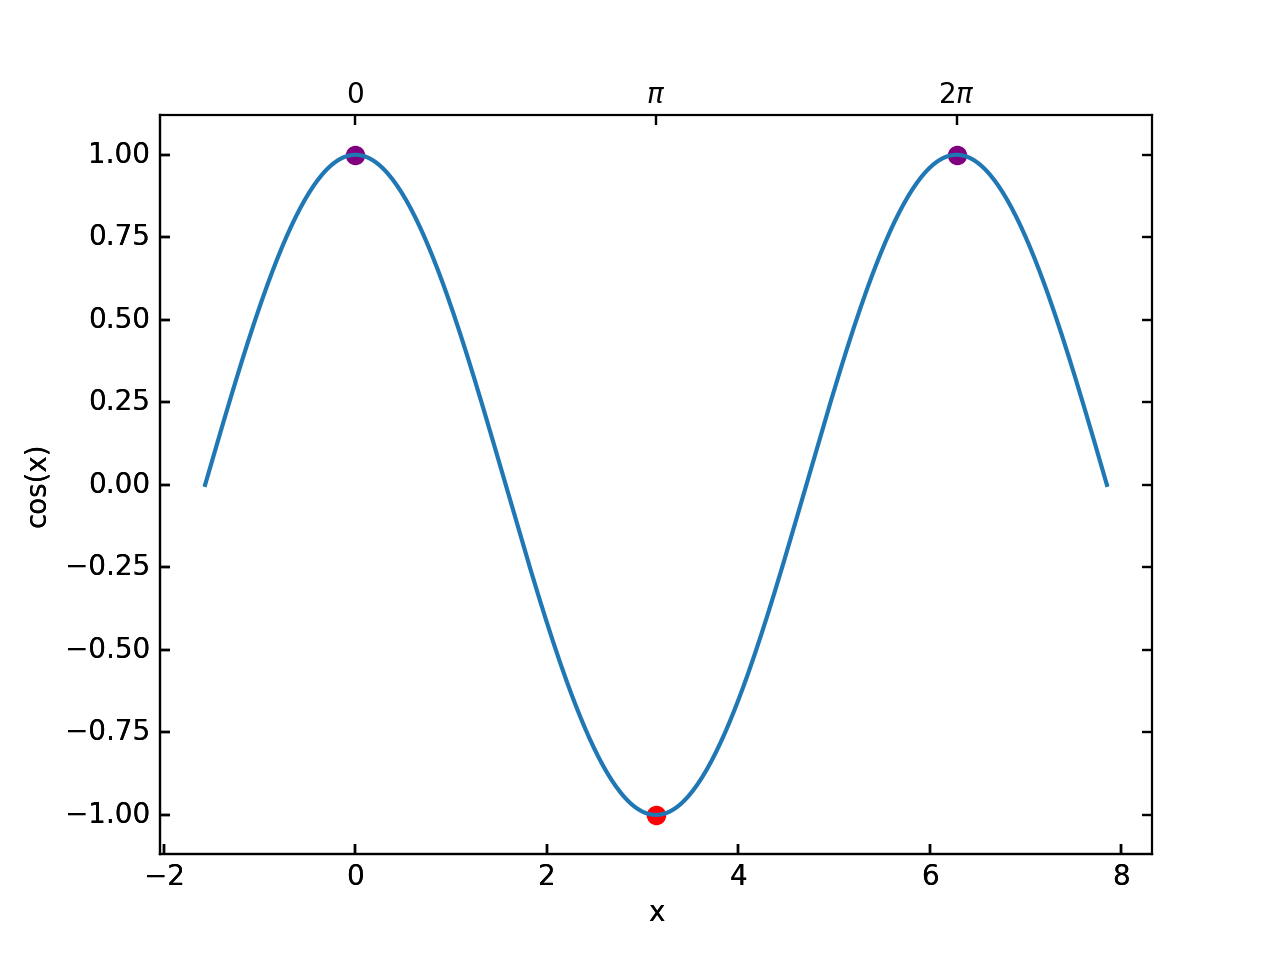
\includegraphics[width=0.8\linewidth]{exp_cosx.png}
\caption{$\cos(x)$}
\label{fig:cost}
\end{figure}

Figure~\ref{fig:cost_contour} demonstrates the distribution of the 2-dimensional cost function in contour. The two purple spots are global minima, and starting from the point ($0, 0$), we can arrive at one of the global minima no matter which direction we choose to go.

\begin{figure}[H]
\begin{center}
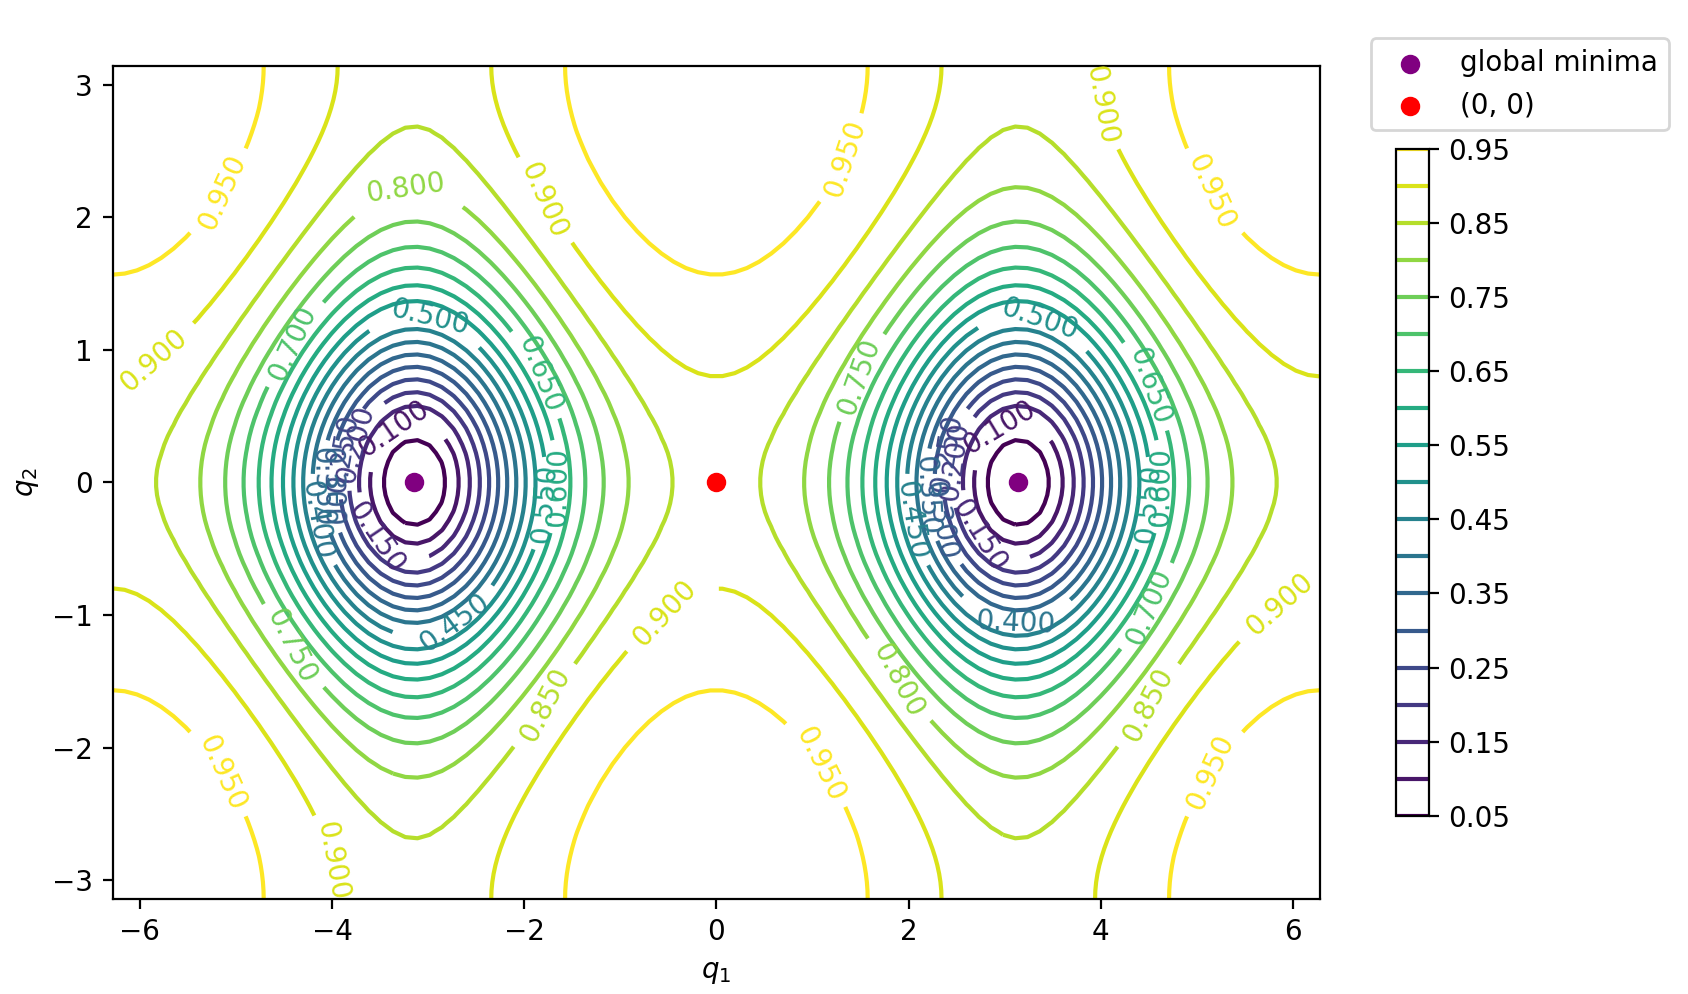
\includegraphics[width=1.1\linewidth]{cost_contour.png}
\caption[caption]{Contour of $1-\exp(-\cos(q_1) + \cos(q_2)-2)$}
\label{fig:cost_contour}
\end{center}
\end{figure}
 In our settings (see Figure~\ref{fig:acrobot}), $q_1$ is the angle between the upper arm and the vertical line going downwards and $q_2$ is the angle between the upper arm and the lower arm. At the beginning of the swing-up process, both arms were hanging downwards so $q_1 = 0$ and $q_2 = 0$ is the starting state. Afterwards, the torque goes into effect so that $q_1$ either increases towards $\pi$ or decreases towards $-\pi$, and the global minima can be achieved in both cases. In other words, the arms can swing up either clockwisely or counter-clockwisely, and both will end up in the desired state. 
\subsection{Lagrangian Constrained Optimization} \label{Lag}
 \quad The constrained trajectory optimization problem in discrete time can be described as below:
\begin{align} & \text{minimize}_{\mathbf x_1,...,\mathbf x_N, u_0,...,u_{N-1}} \sum_{n=0}^{N-1} g(\mathbf x[n], \mathbf u[n]), \nonumber\\
  & \text{subject to} \quad \mathbf x[n+1] = \mathbf {f_d}(\mathbf x[n], \mathbf u[n]) = \mathbf x[n] + \mathbf f(\mathbf x[n], \mathbf u[n]). 
\end{align}
We use Lagrange multipliers to derive the necessary conditions for
our trajectory optimization problem:
\begin{equation}
L(\mathbf x[\cdot],\mathbf u[\cdot],\mathbf \lambda[\cdot]) = \sum_{n=0}^{N-1} g(\mathbf x[n], \mathbf u[n]) +
  \sum_{n=0}^{N-1} \lambda^T[n] \left(\mathbf{f_d}(\mathbf x[n],\mathbf u[n]) - \mathbf x[n+1]\right)
\end{equation}
Take first-order derivatives with respect to $\lambda[\cdot]$, $\mathbf x[\cdot]$ and $\mathbf u[\cdot]$ and set the values equal to $0$'s:

 \begin{align} \forall n\in[0,N-1], \frac{\partial {L}}{\partial{\lambda[n]}} &= \mathbf{f_d}(\mathbf x[n], u[n]) - \mathbf x[n+1] = 0 \nonumber \\ \Rightarrow \mathbf x[n+1] &= \mathbf{f_d}(\mathbf x[n], \mathbf u[n])  \label{eq:dynamic_eq}
 \\
    \forall n\in[0,N-2], \frac{\partial{L}}{\partial \mathbf x[n]} &= \frac{\partial{g(\mathbf x[n],\mathbf u[n])}}{\partial \mathbf x} + \lambda^T[n] \frac{\partial{\mathbf{f_d}(\mathbf x[n],\mathbf u[n])}}{\partial \mathbf x} - \lambda^T[n-1] = 0 \nonumber \\
    \quad \Rightarrow \lambda[n-1] &= \frac{\partial{g(\mathbf x[n],\mathbf u[n])}}{\partial \mathbf x}^T + \frac{\partial{\mathbf{f_d}(\mathbf x[n],\mathbf u[n])}}{\partial \mathbf x}^T \lambda[n]. \label{eq:lambda_i}\\
    \frac{\partial{L}}{\partial \mathbf x[N]} &= -\lambda[N-1] = 0 \nonumber \\ \Rightarrow \lambda[N-1] &= 0 \label{eq:lambda_N}\\
    \forall n\in[0,N-1], \frac{\partial{L}}{\partial \mathbf u[n]} &= \frac{\partial{g(\mathbf x[n]}, \mathbf u[n])}{\partial \mathbf u} + \lambda^T[n] \frac{\partial{\mathbf{f_d}(\mathbf x[n], u[n])}}{\partial \mathbf u} = 0. \label{eq:dldu}
  \end{align}
  
Specifically, 
\begin{align}
\frac{\partial g(\mathbf x[n],\mathbf u[n])}{\partial \mathbf x[n]} &= \begin{bmatrix} -\exp(-k\cos(q_1) + k\cos(q_2) - 2k)\sin(q_1)\\ \exp(-k\cos(q_1) + k\cos(q_2) - 2k)\sin(q_2) \\0\\0 \end{bmatrix}\nonumber \\
\frac{\partial g(\mathbf x[n],\mathbf u[n])}{\partial \mathbf u[n]} &= ru \nonumber \\
\frac{\partial{\mathbf{f_d}(\mathbf x[n],\mathbf u[n])}}{\partial \mathbf x} &= \begin{bmatrix} \mathbf 0 & \mathbf I \\ - \mathbf H^{-1} \frac{{\partial \mathbf G}}{{\partial \mathbf q}}   & -\mathbf H^{-1} {(\mathbf C+ \mathbf I f)}  \end{bmatrix} \nonumber \\
\frac{\partial{\mathbf{f_d}(\mathbf x[n], u[n])}}{\partial \mathbf u} & =  \begin{bmatrix} \mathbf 0 \\ \mathbf 0 \\ \mathbf{H(q)^{-1}B} \end{bmatrix} \nonumber
\end{align}
where 
\begin{align}
\frac{{\partial \mathbf G}}{{\partial \mathbf q}} = \begin{bmatrix} 2g\cos(q_1) + g\cos(q_1+q_2) & g\cos(q_1+q_2)\\
g\cos(q_1+q_2) & g\cos(q_1+q_2) \end{bmatrix} \nonumber
\end{align}
The optimal trajectory should satisfy the conditions that set the above derivatives all equal to zero. \\
\null \quad We tried to solve the above equations using different numerical methods. At first, we used a brute force method that solves all unknowns at one time, but the result failed to converge. With a deeper understanding of the relationship between the variables, we realized what we are looking for is a series of torque $\mathbf{u}[\cdot]$, and the other unknowns can be computed by dynamic functions. Hence, a better way to solve for the unknowns is back-propagation as follows:\\
\null \quad First, suppose we have a series of torques $\mathbf{u}[\cdot]$ that is randomly generated from a normal distribution. Since we already know the initial condition $\mathbf x[0]$, we can infer $\mathbf x[1]$ by Equation~\ref{eq:dynamic_eq}, which is the dynamic equation. In the same manner, we can infer the next state from current state, and thus we can compute $\mathbf x[2], \mathbf x[3], ..., $ $\mathbf x[N-1]$ sequentially. Then we compute the series of $\mathbf \lambda[\cdot]$ in a reverse order: since $\lambda[N-1] = 0$ (Equation~\ref{eq:lambda_N}) and we already know the sequence $\mathbf x[\cdot]$ and $\mathbf u[\cdot]$, by Equation~\ref{eq:lambda_i} we can infer $\lambda[N-1]$. Similarly, we can compute $\lambda[N-2], ..., \lambda[0]$ sequentially.\\
\null \quad Recall that our goal is to find a sequence of torques $\mathbf u[\cdot]$ that satisfies the equation system Equation~\ref{eq:dynamic_eq}, Equation~\ref{eq:lambda_i}, Equation~\ref{eq:lambda_N} and Equation~\ref{eq:dldu}. Now we have reduced the complicated problem with a bunch of unknowns to a typical root-finding one, with the help of the sequential relationship within $\mathbf x[\cdot]$ and $\mathbf \lambda[\cdot]$. Thus we can solve for $\mathbf u[\cdot]$ using Newton's method or other root finding methods.

 \subsection{Chebyshev Approximation}
\quad Theoretically, the torque should change smoothly with time, and hence the values of $\mathbf u[\cdot]$ should be very similar at adjacent time points if the time step is small enough. Therefore, it might be a waste to optimize all of $\mathbf u[\cdot]$ individually, considering the large number of time points we care about. To reduce the dimensions of this problem, we tried to approximate the torque values $\mathbf u[\cdot]$ using polynomial interpolation. The basic idea of polynomial interpolation is to fit a polynomial curve $g(t)$ to the torque values $\mathbf u[\cdot]$ at selected time points.\\
\null \quad In order to minimize the approximation error, we use Chebyshev interpolation \cite{chebyshev}, which is an orthogonal collocation method. In general, Chebyshev interpolation method chooses sample points at Chebyshev points $c_j$ that are calculated using the equation below:
\begin{equation} \label{cheby}
c_j = \cos \left( \frac{(2j - 1)\pi}{2n} \right), j = 1, . . . , n
 \end{equation}
where $n$ is the order of Chebyshev polynomial. By approximating the torque with a polynomial function of time,  now we can describe the torque with as small as $n$ variables instead of a large number of time steps. Moreover, we no longer need to optimize the torque values $\mathbf u[\cdot]$ at each time step, but only need to optimize the torque values $\mathbf w[\cdot]$ at selected Chebyshev points $\mathbf c[\cdot]$. \\
\null \quad To include Chebyshev interpolation in our implementation, we first choose the initial torque values $\mathbf w[\cdot]$ at Chebyshev points $\mathbf c[\cdot]$, and generate the polynomial function $g(t, \mathbf w, \mathbf c)$ with Lagrangian polynomial method \cite{lagrange_interpolation}:
\begin{align} \label{eq:l_i}
 & g(t, \mathbf w, \mathbf c) =\sum_{j=1}^n w_jl_j(t), \nonumber \\
\text{where} \quad
& l_j(t) =\frac{t-c_1}{c_j-c_1}  ... \frac{x-c_{j-1}}{c_j-c_{j-1}} \cdot \frac{x-c_{j+1}}{c_j-c_{j+1}} ...  \frac{x-c_n}{c_j-c_n} \nonumber \\
\end{align}

With $g(t, \mathbf w, \mathbf c)$, we can compute the torque values at each time step $\mathbf u[\cdot]$. Following the steps described in Section~\ref{Lag} we can derive the gradient $\frac{\partial L}{\partial \mathbf u[\cdot]}$. The gradient $\frac{\partial L}{\partial \mathbf w}$ can be calculated with the formula below:
\begin {align}
\frac{\partial L}{\partial \mathbf w} &= \sum_{i = 0}^T g_w(t,\mathbf w, \mathbf c)^T\frac{\partial L}{\partial \mathbf u[i]}, 
\end {align}
where \begin{align}g_w(t,\mathbf w, \mathbf c) & = \begin{bmatrix} l_1(t) \\ l_2(t)\\ ... \\l_n(t) \end{bmatrix}. \nonumber \end{align}
$l_i(t)$ is defined in Equation~\ref{eq:l_i} and $T$ is total number of discrete time steps.
 \subsection{Linear Quadratic Regulator (LQR)}
\null \quad A different way from Lagrangian Constrained Optimization is to use the optimal feedback controller such as Linear Quadratic Regulator (LQR), so long as we can rewrite the cost function in a quadratic form:
\begin{align}
J(\mathbf x_0) =
\int_0^\infty \left[ \mathbf x^T(t) {\mathbf Q} \mathbf x(t) + \mathbf u^T(t) {\mathbf R} \mathbf u(t) \right]dt, \nonumber \\
\text{where}
\quad \mathbf x(0)=\mathbf x_0, {\mathbf Q}={\mathbf Q}^T>0, {\mathbf R}={\mathbf R}^T>0.
\end{align}
Then the optimal control sequence minimizing the cost is given by: 
\begin{align}
\mathbf u(t) &= -\mathbf {Fx}(t), \nonumber\\
\text{where} \quad \mathbf F &= (\mathbf R + \mathbf B^T\mathbf{PB})^{-1}(\mathbf B^T\mathbf{PA} + \mathbf N^T) \nonumber \\
\text{and} \quad \mathbf P &=  \mathbf A^T \mathbf{PA} - \mathbf A^T \mathbf{PB}(\mathbf R+\mathbf B^T \mathbf{PB})^{-1}\mathbf B^T \mathbf{PA} + \mathbf Q 
\end{align}
Detailed explanation please refer to \cite{sontag}.

\section{Results} \label{results}
\subsection{Fully-actuated Acrobot}
\quad To start, we experimented with a fully-actuated acrobot with two actuators, one at the shoulder and the other at the elbow. We tried a variety of ways to solve for the optimal trajectory using Lagrangian constrained optimization method  (as described in Section~\ref{Lag}): Firstly, we tried to solve all the unknowns at once using brute force solver which failed to converge. Then we used the back-propagation way to reduce the number of unknowns and the \texttt{root} function of \texttt{scipy.optimize} module to solve for $\mathbf u$, but sometimes it got to the local maxima instead of minima. Finally we used \texttt{minimum} function of \texttt{scipy.optimize} module and successfully solved for $\mathbf u$ that minimizes our cost function.\\
\null \quad As a warm-up practice for the swing-up task, we solved the stabilization problem first. Using Lagrangian constrained optimization method, we successfully found the trajectory for the fully-actuated acrobot to get back to its balance state ($q_1 = \pi$, $q_2 = 0$) after its upper-arm deviated by an angle of $0.1$ (i.e., $q_1= \pi - 0.1$, $q_2 = 0$) (Figure~\ref{fig:full_stablization}).
\begin{figure}[H]
\begin{center}
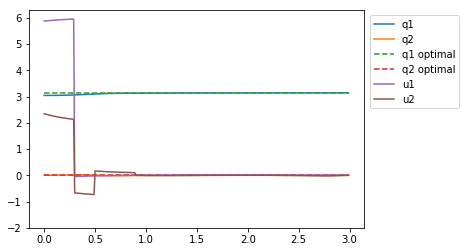
\includegraphics[width=0.8\linewidth]{full_stablization.png}
\caption[caption]{Fully-actuated Stabilization}
\label{fig:full_stablization}
\end{center}
\end{figure}

Then we tried to untangle the swing-up problem of a fully-actuated acrobot. The \texttt{minimum} function of \texttt{scipy.optimize} gets easily trapped in local minima, so we found it difficult to converge to a swing-up trajectory without a good initial value of $\mathbf u$. After many attempts, we finally found a series of initial $\mathbf u$ that can lead to the global minima and can finish the swing-up process (Figure~\ref{fig:full_swingup}).

\begin{figure}[H]
\begin{center}
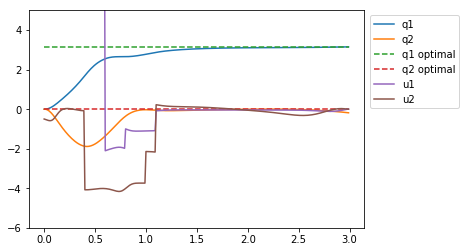
\includegraphics[width=0.8\linewidth]{full_swingup.png}
\caption[caption]{Fully-actuated Swing-up}
\label{fig:full_swingup}
\end{center}
\end{figure}

\subsection{Underactuated Acrobot}
\quad As stated in Section~\ref{Dynamics of the Acrobot}, the dynamic function of underactuated acrobots is identical to that of fully-actuated acrobots except the matrix $\mathbf B = \begin{bmatrix} 0 & 0 \\ 0 & 1 \end{bmatrix}$ instead of $\begin{bmatrix} 1 & 0 \\ 0 & 1\end{bmatrix}$. 
\subsubsection{Stabilization}
\subsubsection{Swing up}
\begin{figure}[H]
\begin{center}
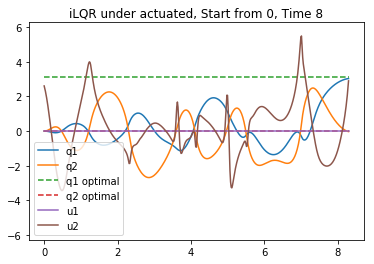
\includegraphics[width=0.6\linewidth]{under_swingup.png}
\caption[caption]{Underactuated Swing-up}
\label{fig:under_swingup}
\end{center}
\end{figure}
\section{Reinforcement Learning} \label{rf}

\newpage
\medskip

\printbibliography
\end{document} to your LaTeX file where you want your
% title page.
%
%%%%%%%%%%%%%%%%%%%%%%%%%%%%%%%%%%%%%%%%%
%\title{Title page with logo}





%----------------------------------------------------------------------------------------
%	PACKAGES AND OTHER DOCUMENT CONFIGURATIONS
%----------------------------------------------------------------------------------------

\documentclass[12pt]{article}
\usepackage[english]{babel}
\usepackage{amsmath}
\usepackage{graphicx}
\usepackage[colorinlistoftodos]{todonotes}
\usepackage{hyperref}
\usepackage[utf8]{inputenc}
\usepackage[backend=bibtex,style=numeric,autocite=plain,sorting=none]{biblatex}
\usepackage{color}
\usepackage{listings}
\usepackage{xcolor}
\usepackage{xparse}
\usepackage{float}

\definecolor{purp}{rgb}{0.6,0.3,0.9}
\addbibresource{citations.bib} %Imports bibliography file

\begin{document}

\begin{titlepage}

\newcommand{\HRule}{\rule{\linewidth}{0.5mm}} % Defines a new command for the horizontal lines, change thickness here

\center % Center everything on the page
 
 %----------------------------------------------------------------------------------------
%	TITLE SECTION
%----------------------------------------------------------------------------------------
\HRule \\[0.4cm]
{\Large \bfseries Optimization in Robotics (Acrobot) Control}\\[0.4cm] % Title of your document
\HRule \\[1.2cm]

%----------------------------------------------------------------------------------------
%	HEADING SECTIONS
%----------------------------------------------------------------------------------------

\textsc{\LARGE Harvard University}\\[1.2cm] % Name of your university/college
\textsc{\Large AM205 Advanced Scientific Computing: Numerical Methods}\\[0.8cm] % Major heading such as course name
\textsc{\large Final Project Report}\\[1.2cm] % Minor heading such as course title


%----------------------------------------------------------------------------------------
%	AUTHOR SECTION
%----------------------------------------------------------------------------------------

\begin{minipage}{0.4\textwidth}
\begin{flushleft} \large
\emph{Authors:}\\
Hengte \textsc{Lin} \\% Your name
Taosha \textsc{Wang}\\
Yifan \textsc{Wang}\\
\end{flushleft}
\end{minipage}
~
\begin{minipage}{0.4\textwidth}
\begin{flushright} \large
\emph{Professor:} \\

Chris H. \textsc{Rycroft} % Supervisor's Name
\end{flushright}
\end{minipage}\\[1cm]

% If you don't want a supervisor, uncomment the two lines below and remove the section above
%\Large \emph{Author:}\\
%John \textsc{Smith}\\[3cm] % Your name

%----------------------------------------------------------------------------------------
%	DATE SECTION
%----------------------------------------------------------------------------------------

{\large \today}\\[1cm] % Date, change the \today to a set date if you want to be precise

%----------------------------------------------------------------------------------------
%	LOGO SECTION
%----------------------------------------------------------------------------------------


\includegraphics[width=0.29\linewidth]{logo.png}\\[1cm] % Include a department/university logo - this will require the graphicx package
 
%----------------------------------------------------------------------------------------

\vfill % Fill the rest of the page with whitespace

\end{titlepage}

%Project motivation: what problem are you trying to solve? What has been
%done before in this area? If appropriate, cite relevant books and papers.

%? 24 points ? Project methods and results: what mathematics and code did you develop
%for your problem? Where appropriate, did you consider mathematical analyses of
%your approach? Is the code that you developed correct?

%? 6 points ? Project conclusions: did you solve what you set out to do? What are
%possible limitations and problems with your approach? How you could you develop
%the project further?
%? 18 points ? Project presentation and organization, divided among the following
%categories:
%? write-up clearly written with good spelling and grammar,
%? figures and tables clear and properly labeled,
%? code well-commented and well-organized.



\begin{abstract}
\quad In this report we describe several algorithms for trajectory optimization of a mechanical system - the acrobot, including the Lagrangian constrained optimization, the linear quadratic regulator, and the Reinforcement Learning algorithm. We tried to solve the stabilization and swing-up problems of the acrobot using each of the algorithms and compared the effectiveness of the results.
\end{abstract}

\section{Introduction}
\quad An \textbf{acrobot}\footnote{A link to an animation of Acrobot: \url{http://www.princeton.edu/~rvdb/WebGL/Acrobot.html} } (in Figure ~\ref{fig:acrobot}) is a planar two-link robotic arm in the vertical plane, typically with an actuator at the elbow (the red point) but no actuator at the shoulder. An acrobot is a typical underactuated robots, which have less actuators than degrees of freedom. The control of underactuated systems has been an interesting topic in robotics industry for it ``gives some reductions of numbers of necessary actuators, of the cost and of the weight of systems" \cite{mingcong}. \\
\begin{figure}[h!]
\centering
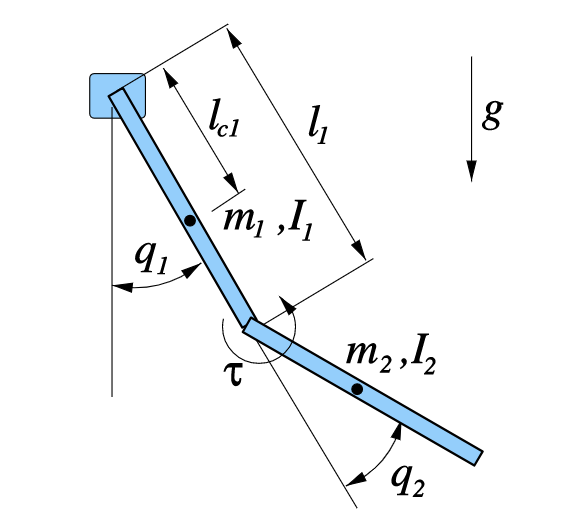
\includegraphics[width=0.45\linewidth]{parameters.png}
\caption{Acrobot (Modified on the basis of picture from \cite{tedrake})}
\label{fig:acrobot}
\end{figure} \\
\null \quad An acrobot closely resembles the movement of a man, and is an important part of a robot. One of the most popular control task studied for the acrobot is the \textit{swing-up} \cite{spong} task, in which the system must use the elbow torque to move the system into a vertical configuration and then balance. Previous studies have proposed many controllers for the Acrobot, such as energy based controllers \cite{1}\cite{2}, controllers based on partiallinearization \cite{1}\cite{3}, tracking controller \cite{4}, back stepping controller \cite{5}, a controller based on the motion of the real gymnast \cite{6} etc. Though optimal control is a powerful framework for specifying complex behaviors with simple objective functions, the computational tools cannot scale well to systems with state dimension more than four or five \cite{tedrake}. In this project, we attempt to find an optimal control solution that is valid from only a single initial condition, instead of solving for the optimal feedback controller for the entire state space. Thus, we represent the optimal control solution as a \textit{trajectory}, \textbf{x($\cdot$)}, \textbf{u($\cdot$)} rather than a feedback control function. \\
\null\quad The rest of this report is organized as follows: In Section~\ref{Dynamics of the Acrobot}, we derive the motion equation of the acrobot using standard, manipulator equation form. In Section~\ref{Optimization}, we set up the Lagrangian equations and derive necessary conditions for the trajectory optimization problem. In Section~\ref{results}, we present the results and runtime analysis of the trajectory optimization solutions. In Section~\ref{rf}, we apply a cutting-edge neural network model - the reinforcement learning algorithm to solve the trajectory optimization problem and compare the performance with traditional methods.

\section{Dynamics of the Acrobot} \label{Dynamics of the Acrobot}
\quad In Figure~\ref{fig:acrobot}, $q_1$ is the shoulder joint angle, $q_2$ is the relative joint angle at the elbow. With the notations in Figure~\ref{fig:acrobot} and let $\mathbf u=[u_1, u_2]^T$ represent the torque applied to the shoulder and the elbow respectively, $\mathbf q = [q_1, q_2]^T$, $\mathbf {\dot q} = [\dot{q_1}, \dot{q_2}]^T$and $\mathbf {\ddot q} = [\ddot{q_1}, \ddot{q_2}]^T$, we can derive the equations of motion in standard, manipulator equation form (for fully actuated acrobot):

\begin{align} \label{eq:manipulator}
\mathbf{H}(\mathbf q) \mathbf{\ddot{q}} +  \mathbf {C( q,\dot{ q})}\mathbf{\dot{q}} + {\mathbf G}(\mathbf q) = \mathbf {Bu} 
\end{align}
where
\begin{align}
{\mathbf H}(\mathbf q) &= \begin{bmatrix} I_1 + I_2 + m_2 l_1^2 + 2m_2 l_1 l_{c2}
  c_2 & I_2 + m_2 l_1 l_{c2} c_2 \\ I_2 + m_2 l_1 l_{c2} c_2 & I_2
  \end{bmatrix},\label{eq:Hacrobot} \nonumber \\
  \mathbf {C(q,\dot{q})} &= \begin{bmatrix} -2 m_2
  l_1 l_{c2} s_2 \dot{q}_2 & -m_2 l_1 l_{c2} s_2 \dot{q}_2 \\ m_2 l_1
  l_{c2} s_2 \dot{q}_1 & 0 \end{bmatrix}, \nonumber \\
{\mathbf G}(\mathbf q) &= \begin{bmatrix} m_1 g l_{c1}s_1 + m_2 g (l_1 s_1 + l_{c2}s_{1+2})
\\ m_2 g l_{c2} s_{1+2} \end{bmatrix}, \nonumber\\
  {\mathbf B} &= \begin{bmatrix} 1 & 0 \\ 0 & 1 \end{bmatrix}. \nonumber
\end{align}
 Note that to model an underactuated acrobot with an actuator at the elbow, we can adjust the above system by simply changing $\mathbf B$ to $\begin{bmatrix} 0 & 0 \\ 0 & 1 \end{bmatrix}$.\\
\null \quad In the next steps we derive the deterministic dynamics from the above motion equations. First, we add frictions $f$ to the system:

\begin{equation} \label{eq:addfriction}
\mathbf {Bu} = \mathbf {B\hat{u}}-f \mathbf{\dot{q}}
\end{equation}
Substituting equation~(\ref{eq:addfriction}) into the right hand side of equation~(\ref{eq:manipulator}), we get:
\begin{equation}
\mathbf{H}(\mathbf q) \mathbf{\ddot{q}} +  \mathbf {C(q,\dot{q})} \mathbf{\dot{q}} + {\mathbf G}(\mathbf q) =  \mathbf {B\hat{u}}-f \mathbf{\dot{q}}
\end{equation}
Afterwards, $\mathbf{\ddot{q}}$ can be calculated as:
\begin{align}
\mathbf{\ddot{q}} &= \mathbf{H(q)}^{-1}[\mathbf{-C(q,\dot{q})\dot{q}-G(q)}+\mathbf {B\hat{u}}-f\mathbf{\dot{q}}] \nonumber \\
&= \mathbf{H(q)}^{-1}[-\mathbf{C(q,\dot{q})\dot{q}}-\mathbf{G(q)}-f\mathbf{\dot{q}}]+\mathbf{H(q)^{-1}B\hat{u}}
\end{align}
Let \textbf{x} = $[q_1, q_2, \dot{q_1}, \dot{q_2}]^T$, we can calculate its derivative with respect to time:
\begin{equation} \label{eq:x_dot}
\mathbf {\dot{x}} = \begin{bmatrix} \dot{q_1} \\ \dot{q_2} \\ \ddot{q_1} \\ \ddot{q_2} \end{bmatrix} = \begin{bmatrix} \dot{q_1} \\ \dot{q_2} \\ \mathbf{H(q)}^{-1}[-\mathbf{C(q,\dot{q})\dot{q}}-\mathbf{G(q)}-f\mathbf{\dot{q}}] \end{bmatrix} 
+ \begin{bmatrix} \mathbf 0 \\ \mathbf 0 \\ \mathbf{H(q)^{-1}B} \end{bmatrix} \mathbf{\hat{u}},
\end{equation}  in the format of 
$
\mathbf{\dot{x}} = \mathbf{f}(\mathbf{ x, u}) = \mathbf{a} + \mathbf {b u}
$. \\
\null \quad For the simplicity of computation, we set all constant values (i.e., $I_1, I_2$, $l_1, l_2, m_1, m_2$, $l_{c1}, l_{c2}$, $c_1$, $c_2$) equal to $1$, hence the matrix $\mathbf{H(q)}$, $\mathbf{C(q,\dot{q})}$ and $\mathbf{G(q)}$ in equation~\ref{eq:x_dot} can be rewritten as:
\begin{align}
\mathbf{H(q)} &= \begin{bmatrix} 3+2\cos(q_2) & 1+\cos(q_2) \\ 1+\cos(q_2) & 1 \end{bmatrix} \nonumber \\
\mathbf{C(q,\dot{q})} &=\begin{bmatrix} -2\sin(q_2)\dot{q_2} & -\sin(q_2)\dot{q_2} \\ \sin(q_2)\dot{q_1} & 0 \end{bmatrix} \nonumber \\
\mathbf{G(q)} &=\begin{bmatrix} g\sin(q_1)+g(\sin(q_1)+\sin(q_1+q_2)) \\ g\sin(q_1+q_2) \end{bmatrix} \nonumber
\end{align}
And hence
\begin{align}
\mathbf{-C(q,\dot{q})\dot{q}-G(q) } &= \begin{bmatrix} 2\sin(q_2)\dot{q_1}\dot{q_2}+\sin(q_2)\dot{q_2}^2 \\ -\sin(q_2)\dot{q_1}^2 \end{bmatrix}-\begin{bmatrix} g\sin(q_1)+g(\sin(q_1)+\sin(q_1+q_2)) \\ g\sin(q_1+q_2) \end{bmatrix} \nonumber \\
&=  \begin{bmatrix} \dot{q_2}(2\dot{q_1}+\dot{q_2})\sin(q_2)-2g \sin(q_1)-g\sin(q_1+q_2) \\ -\dot{q_1}^2\sin(q_2)-g\sin(q_1+q_2) \end{bmatrix} \nonumber
\end{align}

By the end of this section we have derived the $\mathbf{\dot{x}}$ (Equation~\ref{eq:x_dot}). By applying $\mathbf{\dot{x}}$ to the deterministic dynamic function $\mathbf x[n+1] = \mathbf x[n] + \mathbf {\dot{x}}[n]$, we can calculate the next state given previous state and the torque, and hence we have derived the dynamics of the acrobot.

\section{Trajectory Optimization} \label{Optimization}
\subsection{Cost Function}
\quad Define the cost function as
\begin{align}\label{eq:cost}
g(\mathbf q, \mathbf u) = \frac{r}{2}(u_1 + u_2)^2 + 1 - \exp(-k\cos(q_1) + k\cos(q_2) - 2k),
\end{align} where $r, k$ are constants. The reason we choose to use cosine function ($\pm \cos(\cdot)$) as the cost function at both links $q_1$ and $q_2$ is to take advantage of the monotonic and cyclical characteristics of the cosine function. As we can see from Figure~\ref{fig:cost}, $x = \pi$ (the red point) is a global minima, and no matter where we start within the boundary $[0, 2\pi]$ (the purple points), it will converge to $x = \pi$ and will end up with the global minima. \\
\begin{figure}[H]
\centering
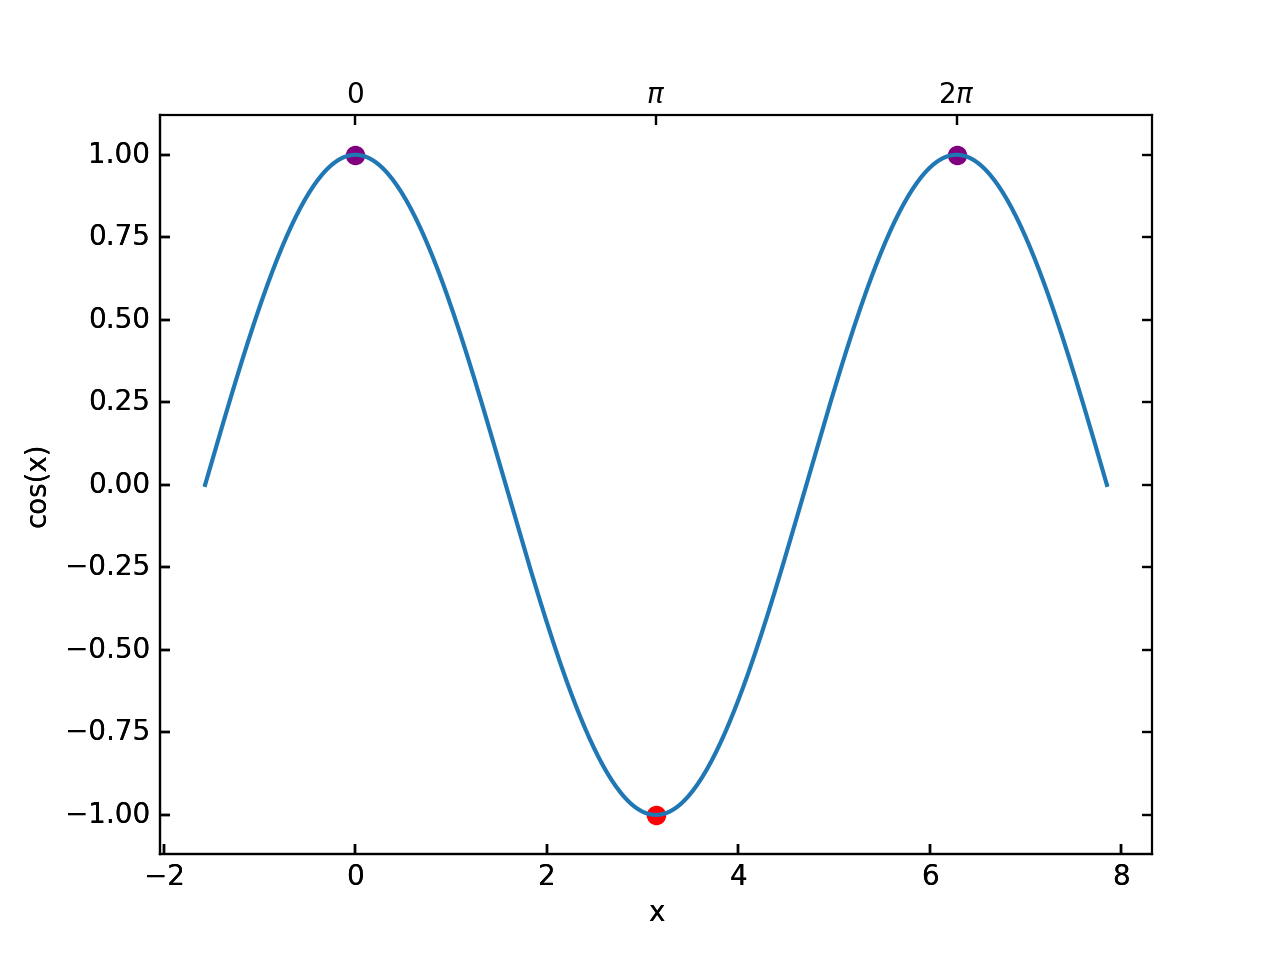
\includegraphics[width=0.8\linewidth]{exp_cosx.png}
\caption{$\cos(x)$}
\label{fig:cost}
\end{figure}

Figure~\ref{fig:cost_contour} demonstrates the distribution of the 2-dimensional cost function in contour. The two purple spots are global minima, and starting from the point ($0, 0$), we can arrive at one of the global minima no matter which direction we choose to go.

\begin{figure}[H]
\begin{center}
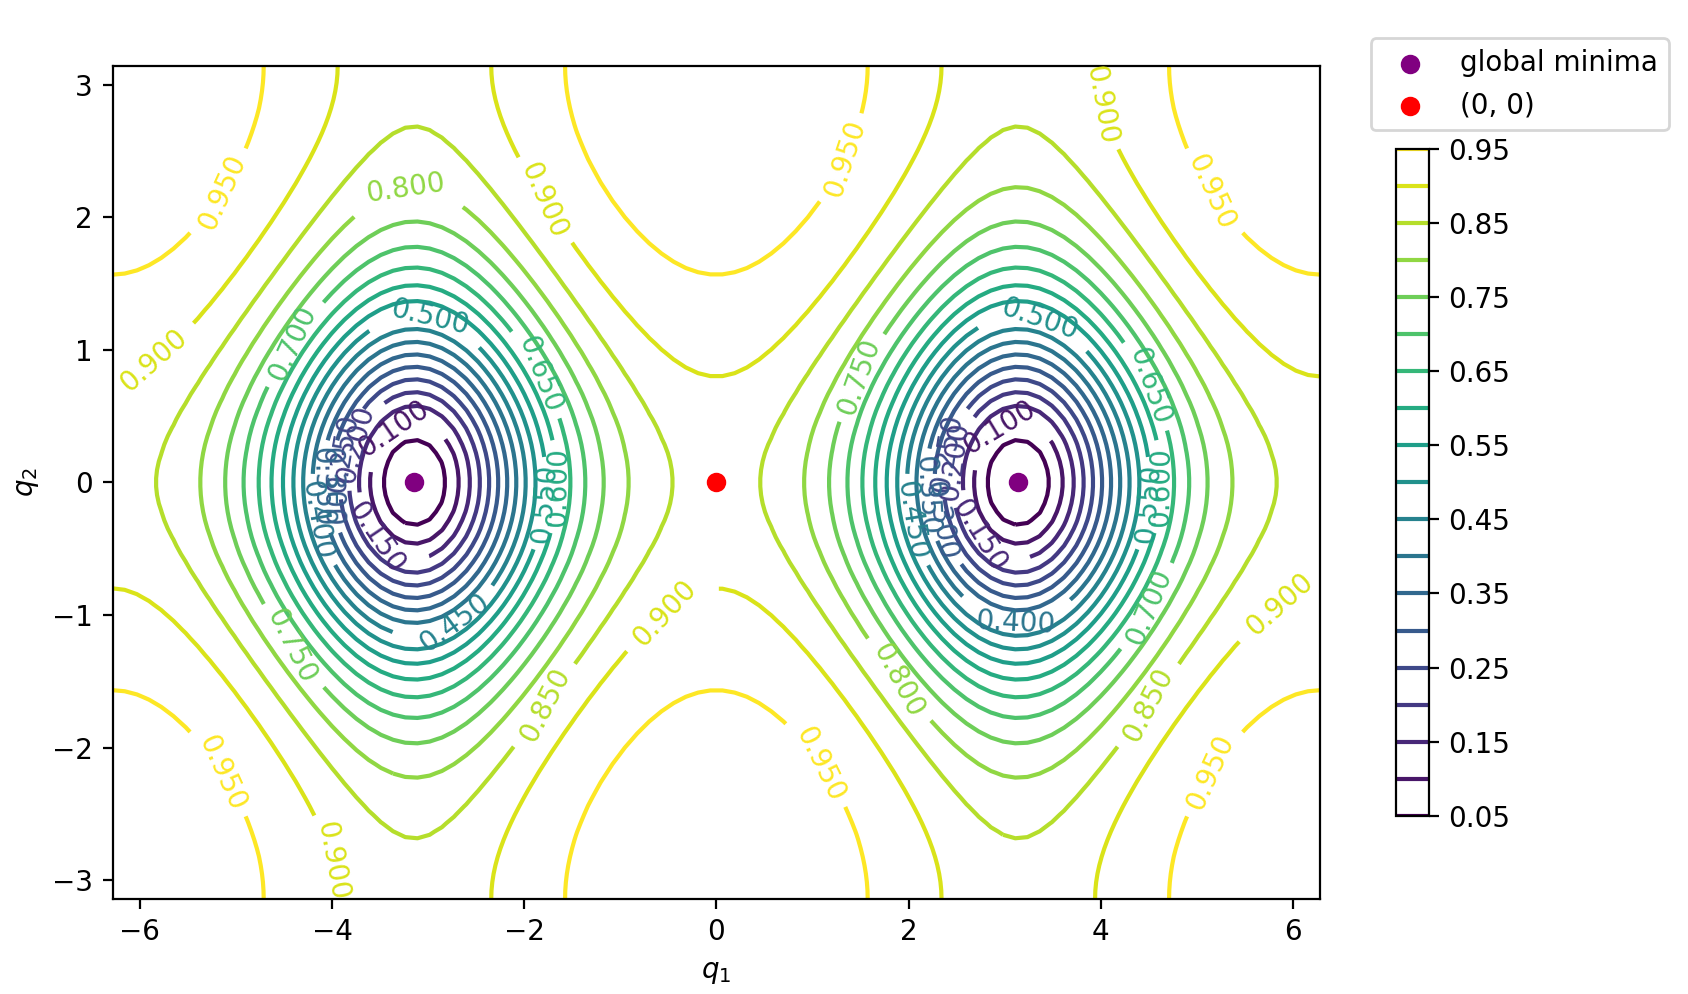
\includegraphics[width=1.1\linewidth]{cost_contour.png}
\caption[caption]{Contour of $1-\exp(-\cos(q_1) + \cos(q_2)-2)$}
\label{fig:cost_contour}
\end{center}
\end{figure}
 In our settings (see Figure~\ref{fig:acrobot}), $q_1$ is the angle between the upper arm and the vertical line going downwards and $q_2$ is the angle between the upper arm and the lower arm. At the beginning of the swing-up process, both arms were hanging downwards so $q_1 = 0$ and $q_2 = 0$ is the starting state. Afterwards, the torque goes into effect so that $q_1$ either increases towards $\pi$ or decreases towards $-\pi$, and the global minima can be achieved in both cases. In other words, the arms can swing up either clockwisely or counter-clockwisely, and both will end up in the desired state. 
\subsection{Lagrangian Constrained Optimization} \label{Lag}
 \quad The constrained trajectory optimization problem in discrete time can be described as below:
\begin{align} & \text{minimize}_{\mathbf x_1,...,\mathbf x_N, u_0,...,u_{N-1}} \sum_{n=0}^{N-1} g(\mathbf x[n], \mathbf u[n]), \nonumber\\
  & \text{subject to} \quad \mathbf x[n+1] = \mathbf {f_d}(\mathbf x[n], \mathbf u[n]) = \mathbf x[n] + \mathbf f(\mathbf x[n], \mathbf u[n]). 
\end{align}
We use Lagrange multipliers to derive the necessary conditions for
our trajectory optimization problem:
\begin{equation}
L(\mathbf x[\cdot],\mathbf u[\cdot],\mathbf \lambda[\cdot]) = \sum_{n=0}^{N-1} g(\mathbf x[n], \mathbf u[n]) +
  \sum_{n=0}^{N-1} \lambda^T[n] \left(\mathbf{f_d}(\mathbf x[n],\mathbf u[n]) - \mathbf x[n+1]\right)
\end{equation}
Take first-order derivatives with respect to $\lambda[\cdot]$, $\mathbf x[\cdot]$ and $\mathbf u[\cdot]$ and set the values equal to $0$'s:

 \begin{align} \forall n\in[0,N-1], \frac{\partial {L}}{\partial{\lambda[n]}} &= \mathbf{f_d}(\mathbf x[n], u[n]) - \mathbf x[n+1] = 0 \nonumber \\ \Rightarrow \mathbf x[n+1] &= \mathbf{f_d}(\mathbf x[n], \mathbf u[n])  \label{eq:dynamic_eq}
 \\
    \forall n\in[0,N-2], \frac{\partial{L}}{\partial \mathbf x[n]} &= \frac{\partial{g(\mathbf x[n],\mathbf u[n])}}{\partial \mathbf x} + \lambda^T[n] \frac{\partial{\mathbf{f_d}(\mathbf x[n],\mathbf u[n])}}{\partial \mathbf x} - \lambda^T[n-1] = 0 \nonumber \\
    \quad \Rightarrow \lambda[n-1] &= \frac{\partial{g(\mathbf x[n],\mathbf u[n])}}{\partial \mathbf x}^T + \frac{\partial{\mathbf{f_d}(\mathbf x[n],\mathbf u[n])}}{\partial \mathbf x}^T \lambda[n]. \label{eq:lambda_i}\\
    \frac{\partial{L}}{\partial \mathbf x[N]} &= -\lambda[N-1] = 0 \nonumber \\ \Rightarrow \lambda[N-1] &= 0 \label{eq:lambda_N}\\
    \forall n\in[0,N-1], \frac{\partial{L}}{\partial \mathbf u[n]} &= \frac{\partial{g(\mathbf x[n]}, \mathbf u[n])}{\partial \mathbf u} + \lambda^T[n] \frac{\partial{\mathbf{f_d}(\mathbf x[n], u[n])}}{\partial \mathbf u} = 0. \label{eq:dldu}
  \end{align}
  
Specifically, 
\begin{align}
\frac{\partial g(\mathbf x[n],\mathbf u[n])}{\partial \mathbf x[n]} &= \begin{bmatrix} -\exp(-k\cos(q_1) + k\cos(q_2) - 2k)\sin(q_1)\\ \exp(-k\cos(q_1) + k\cos(q_2) - 2k)\sin(q_2) \\0\\0 \end{bmatrix}\nonumber \\
\frac{\partial g(\mathbf x[n],\mathbf u[n])}{\partial \mathbf u[n]} &= ru \nonumber \\
\frac{\partial{\mathbf{f_d}(\mathbf x[n],\mathbf u[n])}}{\partial \mathbf x} &= \begin{bmatrix} \mathbf 0 & \mathbf I \\ - \mathbf H^{-1} \frac{{\partial \mathbf G}}{{\partial \mathbf q}}   & -\mathbf H^{-1} {(\mathbf C+ \mathbf I f)}  \end{bmatrix} \nonumber \\
\frac{\partial{\mathbf{f_d}(\mathbf x[n], u[n])}}{\partial \mathbf u} & =  \begin{bmatrix} \mathbf 0 \\ \mathbf 0 \\ \mathbf{H(q)^{-1}B} \end{bmatrix} \nonumber
\end{align}
where 
\begin{align}
\frac{{\partial \mathbf G}}{{\partial \mathbf q}} = \begin{bmatrix} 2g\cos(q_1) + g\cos(q_1+q_2) & g\cos(q_1+q_2)\\
g\cos(q_1+q_2) & g\cos(q_1+q_2) \end{bmatrix} \nonumber
\end{align}
The optimal trajectory should satisfy the conditions that set the above derivatives all equal to zero. \\
\null \quad We tried to solve the above equations using different numerical methods. At first, we used a brute force method that solves all unknowns at one time, but the result failed to converge. With a deeper understanding of the relationship between the variables, we realized what we are looking for is a series of torque $\mathbf{u}[\cdot]$, and the other unknowns can be computed by dynamic functions. Hence, a better way to solve for the unknowns is back-propagation as follows:\\
\null \quad First, suppose we have a series of torques $\mathbf{u}[\cdot]$ that is randomly generated from a normal distribution. Since we already know the initial condition $\mathbf x[0]$, we can infer $\mathbf x[1]$ by Equation~\ref{eq:dynamic_eq}, which is the dynamic equation. In the same manner, we can infer the next state from current state, and thus we can compute $\mathbf x[2], \mathbf x[3], ..., $ $\mathbf x[N-1]$ sequentially. Then we compute the series of $\mathbf \lambda[\cdot]$ in a reverse order: since $\lambda[N-1] = 0$ (Equation~\ref{eq:lambda_N}) and we already know the sequence $\mathbf x[\cdot]$ and $\mathbf u[\cdot]$, by Equation~\ref{eq:lambda_i} we can infer $\lambda[N-1]$. Similarly, we can compute $\lambda[N-2], ..., \lambda[0]$ sequentially.\\
\null \quad Recall that our goal is to find a sequence of torques $\mathbf u[\cdot]$ that satisfies the equation system Equation~\ref{eq:dynamic_eq}, Equation~\ref{eq:lambda_i}, Equation~\ref{eq:lambda_N} and Equation~\ref{eq:dldu}. Now we have reduced the complicated problem with a bunch of unknowns to a typical root-finding one, with the help of the sequential relationship within $\mathbf x[\cdot]$ and $\mathbf \lambda[\cdot]$. Thus we can solve for $\mathbf u[\cdot]$ using Newton's method or other root finding methods.

 \subsection{Chebyshev Approximation}
\quad Theoretically, the torque should change smoothly with time, and hence the values of $\mathbf u[\cdot]$ should be very similar at adjacent time points if the time step is small enough. Therefore, it might be a waste to optimize all of $\mathbf u[\cdot]$ individually, considering the large number of time points we care about. To reduce the dimensions of this problem, we tried to approximate the torque values $\mathbf u[\cdot]$ using polynomial interpolation. The basic idea of polynomial interpolation is to fit a polynomial curve $g(t)$ to the torque values $\mathbf u[\cdot]$ at selected time points.\\
\null \quad In order to minimize the approximation error, we use Chebyshev interpolation \cite{chebyshev}, which is an orthogonal collocation method. In general, Chebyshev interpolation method chooses sample points at Chebyshev points $c_j$ that are calculated using the equation below:
\begin{equation} \label{cheby}
c_j = \cos \left( \frac{(2j - 1)\pi}{2n} \right), j = 1, . . . , n
 \end{equation}
where $n$ is the order of Chebyshev polynomial. By approximating the torque with a polynomial function of time,  now we can describe the torque with as small as $n$ variables instead of a large number of time steps. Moreover, we no longer need to optimize the torque values $\mathbf u[\cdot]$ at each time step, but only need to optimize the torque values $\mathbf w[\cdot]$ at selected Chebyshev points $\mathbf c[\cdot]$. \\
\null \quad To include Chebyshev interpolation in our implementation, we first choose the initial torque values $\mathbf w[\cdot]$ at Chebyshev points $\mathbf c[\cdot]$, and generate the polynomial function $g(t, \mathbf w, \mathbf c)$ with Lagrangian polynomial method \cite{lagrange_interpolation}:
\begin{align} \label{eq:l_i}
 & g(t, \mathbf w, \mathbf c) =\sum_{j=1}^n w_jl_j(t), \nonumber \\
\text{where} \quad
& l_j(t) =\frac{t-c_1}{c_j-c_1}  ... \frac{x-c_{j-1}}{c_j-c_{j-1}} \cdot \frac{x-c_{j+1}}{c_j-c_{j+1}} ...  \frac{x-c_n}{c_j-c_n} \nonumber \\
\end{align}

With $g(t, \mathbf w, \mathbf c)$, we can compute the torque values at each time step $\mathbf u[\cdot]$. Following the steps described in Section~\ref{Lag} we can derive the gradient $\frac{\partial L}{\partial \mathbf u[\cdot]}$. The gradient $\frac{\partial L}{\partial \mathbf w}$ can be calculated with the formula below:
\begin {align}
\frac{\partial L}{\partial \mathbf w} &= \sum_{i = 0}^T g_w(t,\mathbf w, \mathbf c)^T\frac{\partial L}{\partial \mathbf u[i]}, 
\end {align}
where \begin{align}g_w(t,\mathbf w, \mathbf c) & = \begin{bmatrix} l_1(t) \\ l_2(t)\\ ... \\l_n(t) \end{bmatrix}. \nonumber \end{align}
$l_i(t)$ is defined in Equation~\ref{eq:l_i} and $T$ is total number of discrete time steps.
 \subsection{Linear Quadratic Regulator (LQR)}
\null \quad A different way from Lagrangian Constrained Optimization is to use the optimal feedback controller such as Linear Quadratic Regulator (LQR), so long as we can rewrite the cost function in a quadratic form:
\begin{align}
J(\mathbf x_0) =
\int_0^\infty \left[ \mathbf x^T(t) {\mathbf Q} \mathbf x(t) + \mathbf u^T(t) {\mathbf R} \mathbf u(t) \right]dt, \nonumber \\
\text{where}
\quad \mathbf x(0)=\mathbf x_0, {\mathbf Q}={\mathbf Q}^T>0, {\mathbf R}={\mathbf R}^T>0.
\end{align}
Then the optimal control sequence minimizing the cost is given by: 
\begin{align}
\mathbf u(t) &= -\mathbf {Fx}(t), \nonumber\\
\text{where} \quad \mathbf F &= (\mathbf R + \mathbf B^T\mathbf{PB})^{-1}(\mathbf B^T\mathbf{PA} + \mathbf N^T) \nonumber \\
\text{and} \quad \mathbf P &=  \mathbf A^T \mathbf{PA} - \mathbf A^T \mathbf{PB}(\mathbf R+\mathbf B^T \mathbf{PB})^{-1}\mathbf B^T \mathbf{PA} + \mathbf Q 
\end{align}
Detailed explanation please refer to \cite{sontag}.

\section{Results} \label{results}
\subsection{Fully-actuated Acrobot}
\quad To start, we experimented with a fully-actuated acrobot with two actuators, one at the shoulder and the other at the elbow. We tried a variety of ways to solve for the optimal trajectory using Lagrangian constrained optimization method  (as described in Section~\ref{Lag}): Firstly, we tried to solve all the unknowns at once using brute force solver which failed to converge. Then we used the back-propagation way to reduce the number of unknowns and the \texttt{root} function of \texttt{scipy.optimize} module to solve for $\mathbf u$, but sometimes it got to the local maxima instead of minima. Finally we used \texttt{minimum} function of \texttt{scipy.optimize} module and successfully solved for $\mathbf u$ that minimizes our cost function.\\
\null \quad As a warm-up practice for the swing-up task, we solved the stabilization problem first. Using Lagrangian constrained optimization method, we successfully found the trajectory for the fully-actuated acrobot to get back to its balance state ($q_1 = \pi$, $q_2 = 0$) after its upper-arm deviated by an angle of $0.1$ (i.e., $q_1= \pi - 0.1$, $q_2 = 0$) (Figure~\ref{fig:full_stablization}).
\begin{figure}[H]
\begin{center}
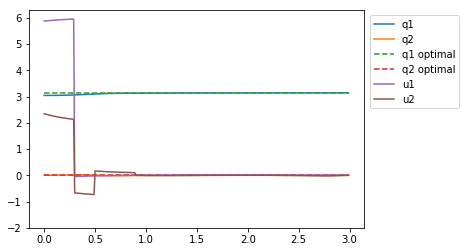
\includegraphics[width=0.8\linewidth]{full_stablization.png}
\caption[caption]{Fully-actuated Stabilization}
\label{fig:full_stablization}
\end{center}
\end{figure}

Then we tried to untangle the swing-up problem of a fully-actuated acrobot. The \texttt{minimum} function of \texttt{scipy.optimize} gets easily trapped in local minima, so we found it difficult to converge to a swing-up trajectory without a good initial value of $\mathbf u$. After many attempts, we finally found a series of initial $\mathbf u$ that can lead to the global minima and can finish the swing-up process (Figure~\ref{fig:full_swingup}).

\begin{figure}[H]
\begin{center}
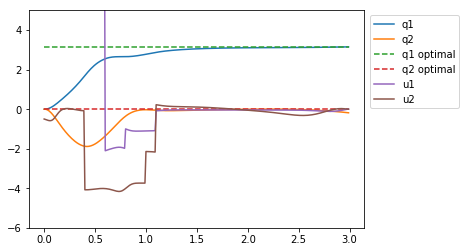
\includegraphics[width=0.8\linewidth]{full_swingup.png}
\caption[caption]{Fully-actuated Swing-up}
\label{fig:full_swingup}
\end{center}
\end{figure}

\subsection{Underactuated Acrobot}
\quad As stated in Section~\ref{Dynamics of the Acrobot}, the dynamic function of underactuated acrobots is identical to that of fully-actuated acrobots except the matrix $\mathbf B = \begin{bmatrix} 0 & 0 \\ 0 & 1 \end{bmatrix}$ instead of $\begin{bmatrix} 1 & 0 \\ 0 & 1\end{bmatrix}$. 
\subsubsection{Stabilization}
\subsubsection{Swing up}
\begin{figure}[H]
\begin{center}
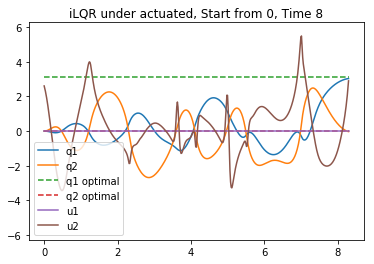
\includegraphics[width=0.6\linewidth]{under_swingup.png}
\caption[caption]{Underactuated Swing-up}
\label{fig:under_swingup}
\end{center}
\end{figure}
\section{Reinforcement Learning} \label{rf}

\newpage
\medskip

\printbibliography
\end{document}